% Note for any github stalkers. I am currently in the process
% of learning LaTeX. I don't know what I'm doing yet. Sorry
% if my code absolutely sucks.

\documentclass{book}

\usepackage{fontspec} % used to import Calibri
\usepackage{anyfontsize} % used to adjust font size

% needed for inch and other length measurements
% to be recognized
\usepackage{calc}

% for colors and text effects as is hopefully obvious
\usepackage[dvipsnames]{xcolor}
\usepackage{soul}

% control over margins
\usepackage[margin=1in]{geometry}
\usepackage[strict]{changepage}

\usepackage{mathtools}
\usepackage{amsfonts}
\usepackage{bm}

\usepackage[scr=rsfs, scrscaled=.96]{mathalpha}

\usepackage{amssymb} % originally imported to get the proof square
\usepackage{xfrac}
\usepackage[overcommands]{overarrows} % Get my preferred vector arrows...
\usepackage{relsize}

% Just am using this to get a dashed line in a table...
% Also you apparently want this to be inactive if you aren't
% using it because it slows compilation.
\usepackage{arydshln} \ADLinactivate 
\newenvironment{allowTableDashes}{\ADLactivate}{\ADLinactivate}

\usepackage{graphicx}
\graphicspath{{./140B_images/}}

\usepackage{tikz}
   \usetikzlibrary{arrows.meta}
   \usetikzlibrary{graphs, graphs.standard}

\usepackage{quiver} %commutative diagrams


\newfontfamily{\calibri}{Calibri}
\setlength{\parindent}{0pt}
\definecolor{RawerSienna}{HTML}{945D27}

% ~~~~~~~~~~~~~~~~~~~~~~~~~~~~~~~~~~~~~~~~~~~~~~~~~~
%Arrow Commands:

% Thank you Bernard, gernot, and Sigur who I copied this from:
% https://tex.stackexchange.com/questions/364096/command-for-longhookrightarrow
\newcommand{\hooklongrightarrow}{\lhook\joinrel\longrightarrow}
\newcommand{\hooklongleftarrow}{\longleftarrow\joinrel\rhook}
\newcommand{\hookxlongrightarrow}[2][]{\lhook\joinrel\xrightarrow[#1]{#2}}
\newcommand{\hookxlongleftarrow}[2][]{\xleftarrow[#1]{#2}\joinrel\rhook}

% Thank you egreg who I copied from:
% https://tex.stackexchange.com/questions/260554/two-headed-version-of-xrightarrow
\newcommand{\longrightarrowdbl}{\longrightarrow\mathrel{\mkern-14mu}\rightarrow}
\newcommand{\longleftarrowdbl}{\leftarrow\mathrel{\mkern-14mu}\longleftarrow}

\newcommand{\xrightarrowdbl}[2][]{%
  \xrightarrow[#1]{#2}\mathrel{\mkern-14mu}\rightarrow
}
\newcommand{\xleftarrowdbl}[2][]{%
  \leftarrow\mathrel{\mkern-14mu}\xleftarrow[#1]{#2}
}

% ~~~~~~~~~~~~~~~~~~~~~~~~~~~~~~~~~~~~~~~~~~~~~~~~~~

\newcommand{\hOne}{%
   \color{Black}%
   \fontsize{14}{16}\selectfont%
}
\newcommand{\hTwo}{%
   \color{MidnightBlue}%
   \fontsize{13}{15}\selectfont%
}
\newcommand{\hThree}{%
   \color{PineGreen!85!Orange}
   \fontsize{13}{15}\selectfont%
}
\newcommand{\hFour}{%
   \color{Cerulean}
   \fontsize{12}{14}\selectfont%
}
\newcommand{\myComment}{%
   \color{RawerSienna}%
   \fontsize{12}{14}\selectfont%
}
\newcommand{\pracOne}{
   \color{BrickRed}%
   \fontsize{13}{15}\selectfont%
}
\newcommand{\pracTwo}{
   \color{Orange}%
   \fontsize{12}{14}\selectfont%
}
\newcommand{\teachComment}{
   \color{Orange}%
   \fontsize{12}{14}\selectfont%
}
\newcommand{\exOne}{%
   \color{Purple}%
   \fontsize{14}{16}\selectfont%
}
\newcommand{\exTwo}{%
   \color{RedViolet}%
   \fontsize{13}{15}\selectfont%
}
\newcommand{\exP}{%
   \color{VioletRed}%
   \fontsize{12}{14}\selectfont%
}
% ~~~~~~~~~~~~~~~~~~~~~~~~~~~~~~~~~~~~~~~~~~~~~~~~

\newcommand{\cyPen}[1]{{\vphantom{.}\color{Cerulean}#1}}
\newcommand{\pinkPen}[1]{{\vphantom{.}\color{VioletRed}#1}}

\newenvironment{myIndent}{%
   \begin{adjustwidth}{2.5em}{0em}%
}{%
   \end{adjustwidth}%
}

\newenvironment{myDindent}{%
   \begin{adjustwidth}{5em}{0em}%
}{%
   \end{adjustwidth}%
}

\newenvironment{myTindent}{%
   \begin{adjustwidth}{7.5em}{0em}%
}{%
   \end{adjustwidth}%
}

\newenvironment{myConstrict}{%
   \begin{adjustwidth}{2.5em}{2.5em}%
}{%
   \end{adjustwidth}%
}

\newcommand{\udefine}[1]{{%
   \setulcolor{Red}%
   \setul{0.14em}{0.07em}%
   \ul{#1}%
}}

\newcommand{\uuline}[2][.]{%
{\vphantom{a}\color{#1}%
\rlap{\rule[-0.18em]{\widthof{#2}}{0.06em}}%
\rlap{\rule[-0.32em]{\widthof{#2}}{0.06em}}}%
#2}

\newcommand*{\markDate}[1]{%
   {\huge \color{Black} \textbf{#1} \newline}%
}

\newcommand*{\markHW}[1]{%
   {\huge \color{Black} \textbf{#1} \newline}%
}

\newcommand{\pprime}{{\prime\prime}}
\newcommand{\ppprime}{{\prime\prime\prime}}
\newcommand{\suchthat}{ \hspace{0.5em}s.t.\hspace{0.5em}}
\newcommand{\rea}[1]{\mathrm{Re}(#1)}
\newcommand{\ima}[1]{\mathrm{Im}(#1)}
\newcommand{\comp}{\mathsf{C}}
\newcommand{\myHS}{ \hspace{0.5em}}
\newcommand{\diam}[1]{\mathrm{diam}(#1)}
\newcommand{\domain}[1]{\mathrm{dom}(#1)}


\newcounter{PropNumber}
\setcounter{PropNumber}{82}
\newcommand{\propCount}[1][1]{%
   \addtocounter{PropNumber}{#1}%
   \thePropNumber%
}
\newcounter{SubPropNumber}
\newcommand{\subPropCount}[1][1]{%
   \addtocounter{SubPropNumber}{1}%
   \theSubPropNumber%
}
\newcommand{\resetSubPropCount}{%
   \setcounter{SubPropNumber}{0}%
}

\newcommand{\myId}{\mathrm{Id}}
\newcommand{\myIm}{\mathrm{im}}
\newcommand{\myObj}{\mathrm{Obj}}
\newcommand{\myHom}{\mathrm{Hom}}
\newcommand{\myEnd}{\mathrm{End}}
\newcommand{\myAut}{\mathrm{Aut}}

\newcommand{\mcateg}[1]{{\bm{\mathsf{#1}}}}

% Thank you Gonzalo Medina and Moriambar who wrote this on stack exchange:
%https://tex.stackexchange.com/questions/74125/how-do-i-put-text-over-symbols%
\newcommand{\myequiv}[1]{\stackrel{\mathclap{\mbox{\footnotesize{$#1$}}}}{\equiv}}

% Thank you chs who wrote this on stack exchange:
%https://tex.stackexchange.com/questions/89821/how-to-draw-a-solid-colored-circle%
\newcommand{\filledcirc}[1][.]{\ensuremath{\hspace{0.05em}{\color{#1}\bullet}\mathllap{\circ}\hspace{0.05em}}}

%Thank you blerbl who wrote this on stack exchange:
%https://tex.stackexchange.com/questions/25348/latex-symbol-for-does-not-divide
\newcommand{\ndiv}{\hspace{-0.3em}\not|\hspace{0.35em}}

\newcommand{\mySepOne}[1][.]{%
   {\noindent\color{#1}{\rule{6.5in}{1mm}}}\\%
}
\newcommand{\mySepTwo}[1][.]{%
   {\noindent\color{#1}{\rule{6.5in}{0.5mm}}}\\%
}

\newenvironment{myClosureOne}[2][.]{%
   \color{#1}%
   \begin{tabular}{|p{#2in}|} \hline \\%
}{%
   \\ \hline \end{tabular}%
}

\newcommand{\fillInBlank}[2][.]{{%
   \color{#1}%
   \rule[-0.12em]{#2em}{0.06em}\rule[-0.12em]{#2em}{0.06em}%
   \rule[-0.12em]{#2em}{0.06em}
}}

\newcommand{\retTwo}{\hfill\bigbreak}

\newcounter{LectureNumber}
\newcommand*{\markLecture}[1]{%
   \stepcounter{LectureNumber}%
   {\huge \color{Black} \textbf{Lecture \theLectureNumber: #1} \newline}%
}

\newcommand{\myVS}{\vphantom{$\int_a^b$}}

% Overarrow stuff:
% ~~~~~~~~~~~~~~~~~~~~~~~~~~~~~~~~~~~~~~~~~~~~~~~~~~~~~~~~~~
\NewOverArrowCommand{myVector}{%
   start = {{\smallermathstyle\relbar}},
   middle = {{\smallermathstyle\relbareda}},
   end={{\rightharpoonup}}, space before arrow=0.15em,
   space after arrow=-0.045em,
}

\NewOverArrowCommand{myBar}{%
   start = {{\relbar}},
   middle = {{\relbar}},
   end={{\relbar}}, space before arrow=0.15em,
   space after arrow=-0.025em,
}

% ~~~~~~~~~~~~~~~~~~~~~~~~~~~~~~~~~~~~~~~~~~~~~~~~~~~~~~~~~~~~

\newcommand{\mVec}[1]{\myVector{#1}}
\newcommand{\mVecAst}[1]{\myVector*{#1}}
\newcommand{\mMat}[1]{\mathbf{#1}}

\title{Math 140B Lecture Notes (Professor: Brandon Seward)}
\author{Isabelle Mills}

\begin{document}
\maketitle{}
\setul{0.14em}{0.07em}
\calibri

\hOne
\markLecture{4/1/2024}

Let $f: E \longrightarrow \mathbb{R}$ where $E \subseteq \mathbb{R}$.

\begin{myIndent}\hTwo
   Since $E$ is the domain of $f$, we shall also refer to it as $\domain{f}$.\retTwo
\end{myIndent}

Fix a point $x \in E \cap E^\prime$. Then consider the function $\frac{f(t)-f(x)}{t-x}$ for $t \in \domain{f}\setminus\{x\}$\\[2pt] and define the \udefine{derivative} of $f$ at $x$ to be $f^\prime(x) = \lim\limits_{t\rightarrow x}\left(\frac{f(t)-f(x)}{t-x}\right)$ provided that this\\[2pt] limit exists. When the above limit exists, we say $f$ is differentiable at $x$. \\ [2pt]

We say $f$ is differentiable on $D \subseteq E$ if $f$ is differentiable at every point in $D$,\\ and if $f$ is differentiable on its entire domain, then we call $f$ \udefine{differentiable}.\retTwo

The function $f^\prime(x) = \lim\limits_{t\rightarrow x}\left(\frac{f(t)-f(x)}{t-x}\right)$ is called the \udefine{derivative} of $f$.\retTwo


{\begin{myIndent}\hTwo
   Proposition \propCount: If $f$ is differentiable at $x$, then $f$ is continuous at $x$.\\ [-10pt]
   
   \begin{myIndent}\hThree
      Proof:\\
      Note that $\lim\limits_{t\rightarrow x}\left(f(t)\right) = \lim\limits_{t\rightarrow x}\left((t-x)\frac{f(t)-f(x)}{t-x} + f(x)\right)$.\\

      Now $\lim\limits_{t\rightarrow x}(t-x) = 0$ and we know $\lim\limits_{t\rightarrow x}\frac{f(t)-f(x)}{t-x} = f^\prime(x)$ exists because $f$ is\\ [3pt] differentiable at $x$. Also, obviously $\lim\limits_{t\rightarrow x}f(x) = f(x)$.\retTwo
      
      Thus by proposition 66 {\color{RawerSienna}(check 140A notes)}, we know that:\\
      
      \begin{tabular}{l}
         $\lim\limits_{t\rightarrow x}\left((t-x)\frac{f(t)-f(x)}{t-x} + f(x)\right) = \lim\limits_{t\rightarrow x}(t-x)\lim\limits_{t\rightarrow x}\left(\frac{f(t)-f(x)}{t-x}\right) + \lim\limits_{t\rightarrow x}f(x)$\\ [3pt]

         $\phantom{\lim\limits_{t\rightarrow x}\left((t-x)\frac{f(t)-f(x)}{t-x} + f(x)\right)} = 0\cdot f^\prime(x) + f(x)$ \\ [-4pt]
         $\phantom{\lim\limits_{t\rightarrow x}\left((t-x)\frac{f(t)-f(x)}{t-x} + f(x)\right)} = f(x)$
      \end{tabular}\retTwo

      Thus, $f$ is continuous at $x$.\retTwo
   \end{myIndent}
\end{myIndent}}


{\begin{center} \teachComment
   \begin{myClosureOne}{5}
      Notes:
      \begin{enumerate}
         \item The above proposition says that differentiability is stronger than\newline continuity.
         \item The converse of this proposition is false. For example, the function\newline $f(x) = |x|$ is continuous at $x = 0$ but not differentiable at\newline $x = 0$.
      \end{enumerate}
   \end{myClosureOne}
\end{center}}

\newpage

{\begin{myIndent}\hTwo
   Proposition \propCount: Suppose $f$ and $g$ are real-valued functions with\\ $\domain{f}, \domain{g} \subseteq \mathbb{R}$. Also suppose $f$ and $g$ are differentiable at $x$. Then\\ $f + g$, $fg$, and (when $g(x) \neq 0$) $\frac{f}{g}$ are differentiable at $x$ with:\\
   
   \begin{tabular}{l c c c c c}
      (A)\quad\quad $(f + g)^\prime(x) = f^\prime(x) + g^\prime(x)$ & &&&&{\hFour(sum rule)} \\ [4pt]
      (B)\quad\quad $(fg)^\prime(x) = f^\prime(x)g(x) + f(x)g^\prime(x)$ & &&&& {\hFour(product rule)} \\ [4pt]
      (C)\quad\quad $\left(\dfrac{f}{g}\right)^\prime\hspace{-0.3em}(x) = \dfrac{f^\prime(x)g(x) - f(x)g^\prime(x)}{(g(x))^2}$ & &&&& {\hFour(quotient rule)}
   \end{tabular}\retTwo

   \begin{myIndent}\hThree
      Proof:
      \begin{myIndent}
         \begin{itemize}
            \item[(A)] Since both $f$ and $g$ are differentiable, we know that both\\ $f^\prime(x) = \lim\limits_{t\rightarrow x}\frac{f(t) - f(x)}{t - x}$ and $g^\prime(x) = \lim\limits_{t\rightarrow x}\frac{g(t) - g(x)}{t - x}$ exist. So\\ by proposition 66:\\ [-11pt]
            
            \hspace{-1.5em}${(f + g)^\prime(x) = \lim\limits_{t\rightarrow x}\frac{f(t) + g(t) - f(x) - g(x)}{t-x} = \lim\limits_{t\rightarrow x}\frac{f(t) - f(x)}{t - x} + \lim\limits_{t\rightarrow x}\frac{g(t) - g(x)}{t - x}}$\\ [4pt]

            This means that $(f + g)^\prime(x) = f^\prime(x) + g^\prime(x)$.\\ [-2pt]

            \item[(B)] Note that:\\
            \begin{tabular}{l}
               $(fg)^\prime(x) = \lim\limits_{t\rightarrow x}\frac{f(t)g(t) - f(x)g(x)}{t-x}$ \\

               $\phantom{(fg)^\prime(x)} = \lim\limits_{t\rightarrow x}\frac{f(t)g(t) \cyPen{\vphantom{.} - f(x)g(t) + f(x)g(t)} - f(x)g(x)}{t-x}$ \\

               $\phantom{(fg)^\prime(x)} = \lim\limits_{t\rightarrow x}\left( g(t)\frac{f(t) - f(x)}{t - x} + f(x)\frac{g(t) - g(x)}{t-x} \right)$
            \end{tabular}\\

            By proposition 83, $g(t) \rightarrow g(x)$ as $t \rightarrow x$. Also, since both $f$\\ and $g$ are differentiable, we know $f^\prime(x) = \lim\limits_{t\rightarrow x}\frac{f(t) - f(x)}{t - x}$ and\\[-2pt] $g^\prime(x) = \lim\limits_{t\rightarrow x}\frac{g(t) - g(x)}{t - x}$ exist. So by proposition 66:\\ [-4pt]

            \hspace{-0.5em}$\lim\limits_{t\rightarrow x}\left( g(t)\frac{f(t) - f(x)}{t - x} + f(x)\frac{g(t) - g(x)}{t-x} \right) = f^\prime(x)g(x) + f(x)g^\prime(x)$.\\

            \item[(C)] Note that:\\
            \begin{tabular}{l}
               $\left(\frac{f}{g}\right)^\prime\hspace{-0.3em}(x) = \lim\limits_{t\rightarrow x}\frac{\frac{f(t)}{g(t)} - \frac{f(x)}{g(x)}}{t - x}$ \\ [2pt]

               $\hphantom{\left(\frac{f}{g}\right)^\prime\hspace{-0.3em}(x)} = \lim\limits_{t\rightarrow x}\left(\frac{1}{g(x)g(t)}\frac{f(t)g(x) - f(x)g(t)}{t - x}\right)$ \\ [8pt]

               $\hphantom{\left(\frac{f}{g}\right)^\prime\hspace{-0.3em}(x)} = \lim\limits_{t\rightarrow x}\left(\frac{1}{g(x)g(t)}\frac{f(t)g(x) \cyPen{\vphantom{.} - f(x)g(x) + f(x)g(x)} - f(x)g(t)}{t - x}\right)$ \\ [8pt]

               $\hphantom{\left(\frac{f}{g}\right)^\prime\hspace{-0.3em}(x)} = \lim\limits_{t\rightarrow x}\left(\frac{1}{g(x)g(t)} \left( g(x)\frac{f(t)-f(x)}{t-x} - f(x)\frac{g(t) - g(x)}{t-x} \right)  \right)$
            \end{tabular}\\ [6pt]
            Now, for the same reasons as before, we can use propositions 83\\ and 66 to separate the parts of the above limit to get that the above limit equals:

            {\centering $\frac{1}{(g(x))^2}\left(g(x)f^\prime(x) - f(x)g^\prime(x)\right)$\par}
         \end{itemize}
      \end{myIndent}
   \end{myIndent}
\end{myIndent}}

\newpage

\exOne

If $f(x) = \alpha$ where $\alpha \in \mathbb{R}$ is constant, then trivially $f^\prime(x) = 0$ for all $x$.\\ Meanwhile, if $f(x) = x$, then we can trivially find that $f^\prime(x) = 1$.\retTwo

Claim 1: For all $n \in \mathbb{Z}_+$, if $f(x) = x^n$, then $f^\prime(x) = nx^{n-1}$.\\ [-15pt]

{\begin{myIndent}\exTwo
   Proof: (we proceed by induction)\retTwo

   Base Case: 
   {\begin{myIndent} \exP
      If $n = 1$, then for $f(x) = x^1$, we have that $f^\prime(x) = 1\cdot x^0$.\retTwo
   \end{myIndent}}

   Induction: 
   {\begin{myIndent}\exP
      Now assume $n > 1$, and for $f(x) = x^{n-1}$, we have that ${f^\prime(x) = (n-1)x^{n-2}\text{.}}$\\ For the rest of this proof, I'll abreviate the derivative of $x^n$ as $(x^n)^\prime$ and the\\ derivative of $x^{n-1}$ as $(x^{n-1})^\prime$. Then using product rule, we know that:\\ [-11pt]

      ${\hspace{-2.5em}(x^n)^\prime = x(x^{n-1})^\prime + 1\cdot x^{n-1} = x\cdot (n-1)x^{n-2} + x^{n-1} = ((n-1) + 1)x^{n-1} = nx^{n-1}}$\retTwo
   \end{myIndent}}
\end{myIndent}}

Claim 2: If $f$ is differentiable at $x$ and $\alpha \in \mathbb{R}$, then $(\alpha f)^\prime(x) = \alpha f^\prime(x)$.\\ [-15pt]

{\begin{myIndent}\exTwo
   Proof:\\ By the product rule: $(\alpha f)^\prime(x) = \alpha f^\prime + (\alpha)^\prime f = \alpha f^\prime + 0\cdot f = \alpha f^\prime$.\retTwo
\end{myIndent}}

These combined with proposition 84 tells us that both polynomials and rational\\ functions are differentiable over their domains.

\mySepTwo

\hOne
{\begin{myIndent}\hTwo
   Proposition \propCount: (chain rule)\\
   Let $f$ and $g$ be real-valued functions with $\domain{f}, \domain{g} \subseteq \mathbb{R}$. Let $x \in \mathbb{R}$.\\ Suppose that $f$ is differentiable at $x$ and that $g$ is differentiable at $f(x)$. Then\\ $g \circ f$ is differentiable at $x$ and $(g \circ f)^\prime(x) = g^\prime(f(x))f^\prime(x)$.\\
   
   {\begin{center}\exTwo
      \begin{myClosureOne}{4.5}
         $\hphantom{.}$\\[-24pt] \ul{Intuition}:
         \begin{myIndent}
            $\lim\limits_{t\rightarrow x}\left(\frac{g(f(t)) - g(f(x))}{\pinkPen{f(t) - f(x)}}\cdot \frac{\pinkPen{f(t)-f(x)}}{t-x}\right) = g^\prime(f(t))\cdot f^\prime(t)$.\newline
         \end{myIndent}

         That said, the issue with this intuition is that we need to\\ address the possibility that $f(t) - f(x) = 0$.\\ [-8pt]
      \end{myClosureOne}\retTwo
   \end{center}}

   {\begin{myIndent}\hThree
      Proof:\\
      Set $y = f(x)$ and define $v(s) = \left\{
      \begin{matrix}
         \frac{g(s) - g(y)}{s-y} - g^\prime(y) & \text{ if } s \neq y \\
         0 & \text{ if } s = y
      \end{matrix}\right.$\retTwo

      Note that $v$ is continuous at $y$. This is because $g$ being differentiable\\ at $f(x) = y$ means that:
      
      {\centering $\lim\limits_{s\rightarrow y}v(s) = \lim\limits_{s\rightarrow y}\left(\frac{g(s) - g(y)}{s-y} - g^\prime(y)\right) = g^\prime(y) - g^\prime(y) = 0 = v(y)$.\retTwo\par}

      \newpage

      Also, since $f$ is differentiable at $x$, we know that $f$ is continuous at $x$.\\ Therefore, $v \circ f$ is continuous at $x$ by proposition 68. Additionally, setting\\ $s = f(t)$, we know that $s \rightarrow y$ as $t \rightarrow x$ because $f$ is continuous at $x$. Thus:

      {\center $ \lim\limits_{t\rightarrow x}v(f(t)) = \lim\limits_{s\rightarrow y}v(s) = 0$ \retTwo\par}
      
      Finally, note that $g(s) - g(y) = (s-y)(g^\prime(y) + v(s))$ for all $s$. Thus by\\ substituting that into our limit:\\ [-8pt]
      \begin{myIndent}
         \begin{tabular}{l}
            $(g \circ f)^\prime(x) = \lim\limits_{t\rightarrow x}\frac{g(f(t)) - g(f(x))}{t - x}$ \\ [8pt]
            $\phantom{(g \circ f)^\prime(x) } = \lim\limits_{t\rightarrow x}\frac{f(t) - f(x)}{t - x}(g^\prime(f(x)) + v(f(t)))$ \\ [8pt]
            $\phantom{(g \circ f)^\prime(x) } = f^\prime(x)\left(g^\prime(f(x)) + 0\right)$\quad\quad (by proposition 66)
         \end{tabular}\retTwo
      \end{myIndent}
   \end{myIndent}}
\end{myIndent}}

\markLecture{4/3/2024}
\exOne\mySepTwo\\ [-12pt]
To start off lecture, here is some intuition about the behavior of derivatives. We'll\\ formally define sine and cosine later (on page \_\_) but for this section please take\\ for granted that $(\sin(x))^\prime = \cos(x)$. Additionally, please take for granted that the\\ power rule holds for non-positive integer exponents.\retTwo

{\begin{myIndent}\exTwo
   \begin{enumerate}
      \item Define $f(x) = \left\{
      \begin{matrix}
         x\sin(\frac{1}{x}) & \text{ if } x \neq 0 \\
         0 & \text{ if } x = 0
      \end{matrix}\right.$\\

      When $x \neq 0$, we have by chain rule that $f^\prime(x) = \sin(\frac{1}{x}) - \frac{1}{x}\cos(\frac{1}{x})$.\\ Meanwhile if $x = 0$, then $\frac{f(t) - f(0)}{t - 0} = \frac{t\sin(\frac{1}{t})}{t} = \sin(\frac{1}{t})$ when $t \neq 0$.\\ So $\lim\limits_{t\rightarrow 0}\left(\frac{f(t) - f(0)}{t - 0}\right)$ does not exist, meaning $f$ is not differentiable at $x$.\\

      This shows that $\domain{f^\prime}$ can be a proper subset of $\domain{f}$.\\

      \item Define $g(x) = \left\{
      \begin{matrix}
         x^2\sin(\frac{1}{x}) & \text{ if } x \neq 0 \\
         0 & \text{ if } x = 0
      \end{matrix}\right.$\\
      
      When $x \neq 0$, we have by chain rule that $g^\prime(x) = 2x\sin(\frac{1}{x}) - \cos(\frac{1}{x})$.\\ Meanwhile when $t \neq 0$:

      {\center $\left|\frac{g(t) - g(0)}{t - 0}\right| = \left|\frac{t^2\sin(\frac{1}{t})}{t}\right| = \left|t\sin(\frac{1}{t})\right| \leq |t|$. \retTwo\par}

      Thus $0 = \lim\limits_{t\rightarrow 0}(-t) \leq \lim\limits_{t\rightarrow 0}\left(\frac{g(t) - g(0)}{t - 0}\right) \leq \lim\limits_{t\rightarrow 0}(t) = 0$, meaning $g^\prime(0) = 0$.\\ [2pt] So $\domain{g^\prime} = \domain{g}$. That said, note that $g^\prime$ has a discontinuity of the\\ [2pt] second kind at $0$. Therefore, this shows that the derivative of a function\\ [2pt] does not have to be continuous.
   \end{enumerate}
\end{myIndent}}

\mySepTwo

\newpage

\hOne Let $X$ be a metric space. A function $f: X \longrightarrow \mathbb{R}$ has a \udefine{local maximum} at $p \in X$\\ if $\exists \delta > 0 \suchthat \forall x \in B_\delta(p),\myHS f(x) \leq f(p)$. Similarly, $f$ has a \udefine{local minimum} if\\ $\exists \delta > 0 \suchthat \forall x \in B_\delta(p),\myHS f(x) \geq f(p)$.\retTwo

{\begin{myIndent}\hTwo
   Proposition \propCount: Let $f: (a, b) \longrightarrow \mathbb{R}$. If $f$ has a local maximum at $x$ and $f$ is\\ differentiable at $x$, then $f^\prime(x) = 0$.\retTwo
   {\begin{myIndent} \hThree
      Proof:\\
      Let $\delta > 0$ so that $\forall t \in B_\delta(x),\myHS f(t) \leq f(x)$. Then for all $t \in (x-\delta, x)$,\\ $\frac{f(t) - f(x)}{t-x} \geq 0$. So $f^\prime(x) \geq 0$. Similarly for all $t \in (x, x+\delta)$, we have\\ $\frac{f(t) - f(x)}{t - x} \leq 0$. Thus $f^\prime(x) \leq 0$.\retTwo

      Hence $f^\prime(x) = 0$.\retTwo

      
      {\begin{myTindent} \hFour
         Note that analogous reasoning can show that if $f$ has a local\\ minimum at $x$ and $f$ is differentiable at $x$, then $f^\prime(x) = 0$.\retTwo
      \end{myTindent}}
   \end{myIndent}}

   Proposition \propCount: If $f, g: [a, b] \longrightarrow \mathbb{R}$ are continuous on $[a, b]$ and differentiable\\ on $(a, b)$, then there exists $x \in (a, b)$ with:
   
   {\centering$(f(b) - f(a))g^\prime(x) = (g(b) - g(a))f^\prime(x)$.\retTwo\par}

   {\begin{myIndent} \hThree
      Proof:\\
      Define $h: [a, b] \longrightarrow \mathbb{R}$ by $h(x) = (f(b) - f(a))g(x) - (g(b) - g(a))f(x)$.\\ Then $h(a) = f(b)g(a) - g(b)f(a) = h(b)$.\retTwo

      Notice that $h$ is continuous on $[a, b]$ and differentiable on $(a, b)$ because of\\ propositions 70 and 84. Since $h^\prime(x) = (f(b) - f(a))g^\prime(x) - (g(b) - g(a))f^\prime(x)$,\\ for all $x \in (a, b)$ it now suffices to show that there exists $x \in (a, b)$ with\\ $h^\prime(x) = 0$.\\
      
      Since $h$ is continuous on a compact set $[a, b]$, we know that $h$ attains a\\ maximum value and a minimum value over the interval $[a, b]$.
      \begin{myDindent}
         \begin{itemize}
            \item[Case 1:] If $h$ is constant on $[a, b]$, then $h^\prime(x) = 0$ for all $x \in (a, b)$.\\ [-8pt]
            \item[Case 2:] If there is $t \in (a, b)$ with $h(t) > h(a) = h(b)$, then $h(a)$ and\\ $h(b)$ can't be the max. value that $h$ attains on $[a, b]$. So $h$ has a maximum at some point $x \in (a, b)$. Then by the last theorem,\\ $h^\prime(x) = 0$.
            \item[Case 3:] If there is $t \in (a, b)$ with $h(t) < h(a) = h(b)$, then $h(a)$ and\\ $h(b)$ can't be the min. value that $h$ attains on $[a, b]$. So $h$ has a minimum at some point $x \in (a, b)$. Then by the last theorem,\\ $h^\prime(x) = 0$.
         \end{itemize}
      \end{myDindent}
   \end{myIndent}}

   \newpage

   Proposition \propCount: (Mean Value Theorem)\\
   If $f: [a, b] \longrightarrow \mathbb{R}$ is continuous on $[a, b]$ and differentiable on $(a, b)$, then there is\\ $x \in (a, b)$ with $f(b) - f(a) = (b - a)f^\prime(x)$.\retTwo
   
   {\begin{myIndent} \hThree
      To prove this, apply the previous proposition with $g(x) = x$.\retTwo
   \end{myIndent}}

   Proposition \propCount: Suppose $f (a, b) \longrightarrow \mathbb{R}$ is differentiable. Then:
   \begin{itemize}
      \item If $f^\prime(x) \geq 0$ for all $x \in (a, b)$, then $f$ is monotone increasing.
      \item If $f^\prime(x) \leq 0$ for all $x \in (a, b)$, then $f$ is monotone decreasing.
      \item If $f^\prime(x) = 0$ for all $x \in (a, b)$, then $f$ is constant.\retTwo
   \end{itemize}

   
   \begin{myIndent}\hThree
      Proof:\\
      For all $a < x_1 < x_2 < b$, we know by the mean value theorem that there\\ exists $t \in (x_1, x_2)$ with $f(x_2) - f(x_1) = (x_2 - x_1)f^\prime(t)$. Then since\\ $x_2 - x_1 > 0$, the sign of $f(x_2) - f(x_1)$ depends entirely on $f^\prime(t)$.\retTwo
   \end{myIndent}
\end{myIndent}}

\mySepTwo

\markLecture{4/5/2024}

Even though derivatives are not necessarily continuous, we can show they always\\ satisfy the conclusion of the intermediate value theorem.

{\begin{myIndent}\hTwo
   Proposition \propCount: Suppose $f: [a, b] \rightarrow \mathbb{R}$ is differentiable and $\lambda \in \mathbb{R}$ satisfies\\ that $f^\prime(a) < \lambda < f^\prime(b)$. Then there is $x \in (a, b)$ with $f^\prime(x) = \lambda$.\\
   
   {\begin{myIndent}\hThree
      Proof:\\
      Define $g: [a, b] \rightarrow \mathbb{R}$ by the rule $g(t) = f(t) - \lambda t$. Then $g$ is\\ differentiable with $g^\prime(t) = f^\prime(t) - \lambda$. So, it suffices to find\\ $x \in (a, b)$ with $g^\prime(x) = 0$\retTwo

      Since $g$ is differentiable, we know that $g$ is continuous. Adding in\\ the fact that $[a, b]$ is compact, we know that $g$ achieves a minimum\\ value. So, let $x \in [a, b]$ be such that $g(x)$ is the minimum value of $g$.\retTwo

      Now consider that $f^\prime(a) < \lambda < f^\prime(b) \Longrightarrow g^\prime(a) < 0 < g^\prime(b)$. Since\\ $g^\prime(a) < 0$, there is some $t_1 > a$ near $a$ such that $g(x) \leq g(t_1) < g(a)$.\\ [-11pt]
      {\begin{myIndent}\hFour
         Explanation:\\
         Set $\varepsilon = |g^\prime(a)|$. Then by the definition of limits:
         
         {\centering $\exists \delta > 0 \suchthat \forall t \in (a, a + \delta), \myHS \left|\frac{g(t)- g(a)}{t - a} - g^\prime(a)\right| < \varepsilon$.\retTwo\par}

         Then because $g^\prime(a)$ is negative, we must have that $\frac{g(t)- g(a)}{t - a} < 0$.\\ But as $t - a > 0$, we must have that $g(t)- g(a) < 0$.
         {\begin{myTindent}\begin{myIndent}\teachComment
            This will be a common trick so get used to it.
         \end{myIndent}\end{myTindent}}
      \end{myIndent}}

      \newpage

      Similarly, since $g^\prime(b) > 0$, there is some $t_2 < b$ near $b$ such that\\ $g(x) \leq g(t_2) < g(b)$. Hence, we have shown that $x \neq a$ and $x \neq b$,\\ meaning that $x \in (a, b)$. Then, by applying proposition 86 we know\\ that $g^\prime(x) = 0$.\retTwo


      \begin{myDindent} \teachComment
         We can prove an analogous theorem for when $f^\prime(b) < \lambda < f^\prime(a)$.\retTwo
      \end{myDindent}
   \end{myIndent}}

   \uuline{Corollary}: If $f: [a, b] \longrightarrow \mathbb{R}$ is differentiable, then $f^\prime$ has no simple discontinuities.\\
   
   {\begin{myIndent}\hThree
      Proof:\\
      Assume that $x \in [a, b)$ and $f^\prime(x+)$ exists. Then let $\varepsilon > 0$. By the definition\\ of $f(x+)$:
      
      {\centering$\exists \delta > 0 \suchthat \forall t \in (x, x + \delta),\myHS |f^\prime(t) - f^\prime(x+)| < \sfrac{\varepsilon}{2}$.\retTwo\par}
      
      If $f^\prime(t) = f^\prime(x)$ for all $t \in (x, x+\delta)$, then we automatically have that\\ $f^\prime(x+) = f^\prime(x)$. So assume there exists $t \in (x, x+\delta)$ such that\\ $f^\prime(t) \neq f^\prime(x)$. Then by the previous proposition, there exists $s \in (x, t)$\\ such that $f^\prime(s)$ is between $f^\prime(x)$ and $f^\prime(t)$, and that $|f^\prime(s) - f^\prime(x)| < \sfrac{\varepsilon}{2}$.\\ Finally:

      {\centering $|f^\prime(x) - f^\prime(x+)| \leq |f^\prime(x) - f^\prime(s)| + |f^\prime(s) - f^\prime(x+)| < \sfrac{\varepsilon}{2} + \sfrac{\varepsilon}{2} = \varepsilon$.\retTwo\par}

      So $f^\prime(x)$ must equal $f^\prime(x+)$. Similarly, we can show that if $x \in (a, b]$ and\\ $f^\prime(x-)$ exists, then $f^\prime(x) = f^\prime(x-)$. Thus, it is impossible for $f^\prime$ to have a\\ simple discontinuity.\retTwo

      {\begin{myDindent}\teachComment
         However, we already saw that $f^\prime$ can have discontinuities of the\\ second kind.\retTwo
      \end{myDindent}}
   \end{myIndent}}

   Proposition \propCount: (L'Hôpital's rule)\\
   Suppose $-\infty \leq a \leq b \leq +\infty$, that $f, g: (a, b) \longrightarrow \mathbb{R}$ are differentiable, and that\\ $\forall x \in (a, b), \myHS g^\prime(x) \neq 0$. Then suppose that $\lim\limits_{x\rightarrow a}\frac{f^\prime(x)}{g^\prime(x)} = A \in \mathbb{R} \cup \{-\infty, \infty\}$.\\ If either:
   \begin{itemize}
      \item both $f(x) \rightarrow 0$ and $g(x) \rightarrow 0$ as $x \rightarrow a$
      \item or either $g(x) \rightarrow +\infty$ or $g(x) \rightarrow -\infty$ as $x \rightarrow a$
   \end{itemize}
   then $\lim\limits_{x\rightarrow a}\frac{f(x)}{g(x)}\rightarrow A$.\hspace{11em}{\teachComment (A similar result holds as $x \rightarrow b$.)}\\

   {\begin{myIndent}\hThree
      Proof:\\
      Since $A \in \mathbb{R} \cup \{-\infty, \infty\}$, to show that $\lim\limits_{x\rightarrow a}\frac{f(x)}{g(x)} = A$, it suffices to show:
      \begin{enumerate}
         \item If $A \neq +\infty$, then for every $q \in \mathbb{R}$ with $q > A$, there is $c > a$ with\\ $\forall x \in (a, c),\myHS \frac{f(x)}{g(x)} < q$.
         \item If $A \neq -\infty$, then for every $q \in \mathbb{R}$ with $q < A$, there is $c > a$ with\\ $\forall x \in (a, c),\myHS \frac{f(x)}{g(x)} > q$
      \end{enumerate}

      \newpage

      Let's prove requirement 1. Assume $A \neq +\infty$ and fix $q \in \mathbb{R}$ with $q > A$.\\
      Next pick $r \in \mathbb{R}$ with $A < r < q$. Since $\frac{f^\prime(x)}{g^\prime(x)} \rightarrow A$ as $x \rightarrow a$, there is\\ [-3pt] $c_1 > a$ with $\forall x \in (a, c_1), \myHS \frac{f^\prime(x)}{g^\prime(x)} < r$.\retTwo
      
      Now consider that whenever $a < x < y < c_1$, we have by proposition 87\\ that there exists $t \in (x, y)$ such that:

      {\center $ (f(y) - f(x))g^\prime(t) = (g(y) - g(x))f^\prime(t)$.\retTwo\par}

      By the hypothesis of the theorem, $g^\prime(t)$ can't be zero. Aditionally, because\\ of the mean value theorem, if $g(y) - g(x) = 0$, then there would have to\\ exist $s \in (x, y)$ with $g^\prime(s) = 0$, thus contradicting the hypothesis of the\\ theorem. So, it is safe to rearrange the above expression to get that:

      {\center $\frac{f(y) - f(x)}{g(y) - g(x)} = \frac{f^\prime(t)}{g^\prime(t)} < r$ \retTwo\par}

      
      Case 1: Assume $f(x) \rightarrow 0$ and $g(x) \rightarrow 0$ as $x \rightarrow a$.
      {\begin{myIndent}\hFour
         Then fixing any $y \in (a, c_1)$, we have that $\lim\limits_{x\rightarrow a}\frac{f(y) - f(x)}{g(y) - g(x)} = \frac{f(y)}{g(y)} \leq r < q$.\retTwo
      \end{myIndent}}

      Case 2: Assume $g(x) \rightarrow +\infty$ or $g(x) \rightarrow -\infty$ as $x \rightarrow a$.
      {\begin{myIndent}\hFour
         Then fix any $y \in (a, c_1)$ and pick $c_2 \in (a, c_1)$ such that $\forall x \in (a, c_2)$,\\ $g(x)$ and $g(x) - g(y)$ have the same sign. Then, $\forall x \in (a, c_2)$, we have\\ that $\frac{g(x) - g(y)}{g(x)} > 0$. So:

         {\center $ \frac{f(y) - f(x)}{g(y) - g(x)}\cdot\frac{g(x) - g(y)}{g(x)} < r \cdot \frac{g(x) - g(y)}{g(x)} $ \retTwo\par}

        Note that $\frac{f(y) - f(x)}{g(y) - g(x)}\cdot\frac{g(x) - g(y)}{g(x)} = \frac{f(x) - f(y)}{g(x)} = \frac{f(x)}{g(x)} - \frac{f(y)}{g(x)}$ and\\ $\frac{g(x) - g(y)}{g(x)} = 1 - \frac{g(y)}{g(x)}$. Thus, we can rearrange terms to get that:\\ [-8pt]

         {\center $ \frac{f(x)}{g(x)} < \left(1 - \frac{g(y)}{g(x)}\right)r + \frac{f(y)}{g(x)}$ \retTwo\par}

         Now, $\lim\limits_{x\rightarrow a}\left(\left(1 - \frac{g(y)}{g(x)}\right)r + \frac{f(y)}{g(x)}\right) = (1 - 0)r + 0 = r$. So, there is\\ $c_3 \in (a, c_2)$ such that $\forall x \in (a, c_3), \myHS \left(1 - \frac{g(y)}{g(x)}\right)r + \frac{f(y)}{g(x)} < q$.\retTwo

         Hence, $\forall x \in (a, c_3)$, $\frac{f(x)}{g(x)} < q$.\retTwo
      \end{myIndent}}
      
      Requirement 2 is proved in a similar fashion. $\blacksquare$\retTwo
   \end{myIndent}}
\end{myIndent}}

Let $f$ be a real-valued function with $\domain{f} \subseteq \mathbb{R}$. If $f^\prime$ is defined and is itself\\ differentiable, then the derivative of $f^\prime$ is denoted $f^\pprime$ and called the \udefine{second\\ derivative} of $f$. We similarly define $f^{\ppprime}, f^{(4)}, \ldots, f^{(n)}$.\retTwo

Also, we shall sometimes use $f^{(0)}$ to refer to the original function $f$.

\newpage

\markLecture{4/8/2024}

{\begin{myIndent}\hTwo
   Proposition \propCount: (Taylor's Theorem)\\
   Suppose that $f: [a, b] \longrightarrow \mathbb{R}$, that $f^{(n-1)}$ is continuous on $[a, b]$, and that $f^{(n)}$ is\\ defined on $(a, b)$. Then pick $\alpha \in [a, b]$ and define:

   {\centering $P(t) = \sum\limits_{k=0}^{n-1}\frac{f^{(k)}(\alpha)}{k!}(t - \alpha)^k$\retTwo\par}

   Then for every $\beta \in [a, b] \setminus \{\alpha\}$, there is some $x$ between $\alpha$ and $\beta$ such that\\ $f(\beta) = P(\beta) + \frac{f^{(n)}(x)}{n!}(\beta - \alpha)^n$.\\ [-6pt]

   {\begin{myIndent}\hThree
      Proof:\\
      Set $M = \frac{f(\beta) - P(\beta)}{(\beta - \alpha)^n}$ so that $f(\beta) = P(\beta) + M(\beta - \alpha)^n$. Having done that,\\ [-5pt] our goal is now to find an $x$ between $\alpha$ and $\beta$ such that $\frac{f^{(n)}(x)}{n!} = M$. \retTwo

      Define $g(t) = f(t) - P(t) - M(t - \alpha)^n$. Then, since $P$ is a polynomial\\ of degree $n - 1$, we have that $P^{(n)}(t) = 0$ for all $t$. So:
      
      {\centering $g^{(n)}(t) = f^{(n)}(t) - Mn!$\retTwo\par}

      Thus, it suffices to find an $x$ between $\alpha$ and $\beta$ such that $g^{(n)}(x) = 0$.\retTwo

      Importantly, $P$ is the unique polynomial of degree $n - 1$ satisfying for all\\ $0 \leq k \in \leq k-1$ that $P^{(k)}(\alpha) = f^{(k)}(\alpha)$. Thus, for all $0 \leq k \in \leq k-1$, we\\ have that:
      
      {\centering$g^{(k)}(\alpha) = f^{(k)}(\alpha) - P^{(k)}(\alpha) - M\frac{n!}{(n-k)!}(\alpha - \alpha)^{n-k} = 0$.\retTwo\par}
      
      At the same time, for all $0 \leq k \leq n-1$, we know that $g^{(k)}$ is continuous\\ on $[\alpha, \beta]$ and differentiable on $(\alpha, \beta)$. So, we shall proceed by repeatedly\\ applying the mean value theorem.
      \begin{myIndent}
         \begin{itemize}
            \item $g(\beta) = 0$ and $g(\alpha) = 0$. So, there is $x_1$ between $\alpha$ and $\beta$\\ with $g^\prime(x_1) = 0$.
            \item $g^\prime(x_1) = 0$ and $g^\prime(\alpha) = 0$. So, there is $x_2$ between $\alpha$ and $x_1$\\ with $g^\pprime(x_2) = 0$.
            
            {\centering\fontsize{18}{0}\selectfont $\vdots\phantom{aaaaaaa}$ \retTwo\par}
         \end{itemize}
      \end{myIndent}

      Eventually, you will get an $x_n$ between $\alpha$ and $x_{n-1}$ with $g^{(n)}(x_n) = 0$. $\blacksquare$\retTwo

      \begin{myTindent}\teachComment
         Note that this can be interpretted as a higher order analog\\ of the mean value theorem. In fact, if $n = 1$ then this is\\ just the mean value theorem.
      \end{myTindent}
   \end{myIndent}}
\end{myIndent}}

\newpage

The limit definition of the derivative still makes sense and can be applied to\\ situations where $f$ is a $\mathbb{C}$-valued or $\mathbb{R}^k$-valued function. Although, because\\ this class is called "real" analysis, we shall always require that $\domain{f} \subseteq \mathbb{R}$.
{\begin{myTindent}\begin{myTindent}\teachComment
   (We will talk in 140C about when $\domain{f} \subseteq \mathbb{R}^k$)\retTwo
\end{myTindent}\end{myTindent}}

If $f$ is a $\mathbb{C}$-valued function, then we can write that $f = f_1 + if_2$ where $f_1$ and\\ $f_2$ are real-valued. Then, $f$ is differentiable if and only if $f_1$ and $f_2$ are\\ differentiable. Also, $f^\prime(x) = f_1^\prime(x) + if_2^\prime(x)$.\retTwo

{\begin{myIndent}\exTwo\color{Purple}
   Proof:\\
   Firstly consider any sequence $(x_n)$ such that $x_n \rightarrow x$ as $n \rightarrow \infty$ but $x_n \neq x$ for\\ any $n$. Then assuming  $f^\prime(x)$ exists, we know that:

   {\centering $\lim\limits_{n\rightarrow\infty}\left|\frac{f(x_n) - f(x)}{x_n-x} - f^\prime(x)\right| = 0$ \retTwo\par}

   Now importantly:
   {\begin{itemize}\exP\color{RedViolet}
      \item $0 \leq \left|\frac{f_1(x_n) - f_1(x)}{x_n - x} - \rea{f^\prime(t)}\right| = \left|\mathrm{Re}\hspace{-0.24em}\left(\frac{f(x_n) - f(x)}{x_n - x} - f^\prime(x) \right)\right| \leq \left|\frac{f(x_n) - f(x)}{x_n-x} - f^\prime(x)\right|$
      \item $0 \leq \left|\frac{f_2(x_n) - f_2(x)}{x_n - x} - \ima{f^\prime(t)}\right| = \left|\mathrm{Im}\hspace{-0.24em}\left(\frac{f(x_n) - f(x)}{x_n - x} - f^\prime(x) \right)\right| \leq \left|\frac{f(x_n) - f(x)}{x_n-x} - f^\prime(x)\right|$\\
   \end{itemize}}

   So, ${\fontsize{12}{14}\selectfont\lim\limits_{n\rightarrow\infty}\left|\frac{f_1(x_n) - f_1(x)}{x_n-x} - \rea{f^\prime(x)}\right| = 0}$ and ${\fontsize{12}{14}\selectfont\lim\limits_{n\rightarrow\infty}\left|\frac{f_2(x_n) - f_2(x)}{x_n-x} - \ima{f^\prime(x)}\right| = 0}$.\\ [2pt]
   This means $f_1^\prime(x)$ and $f_2^\prime(x)$ exist with $f_1^\prime(x) = \rea{f^\prime(x)}$ and $f_2^\prime(x) = \ima{f^\prime(x)}$.\retTwo

   Meanwhile, assume that $f_1^\prime(x)$ and $f_2^\prime(x)$ exist. Then:

   {\centering\exP\color{RedViolet} 
   \begin{tabular}{l}
      $f^\prime(x) = \lim\limits_{t\rightarrow x}\left(\frac{f_1(t) + if_2(t) - f_1(x) - if_2(x)}{t - x}\right)$\\ [3pt]
      $\phantom{f^\prime(x) } = \lim\limits_{t\rightarrow x}\left(\frac{f_1(t) - f_1(x)}{t - x} + i\frac{f_2(t) - f_2(x)}{t-x}\right) =   f_1^\prime(x) + if_2^\prime(x)$.
   \end{tabular}
   \retTwo\par}
\end{myIndent}}


Similarly, if $\mVec{f}$ is $\mathbb{R}^k$-valued, then we can write $\mVec{f} = (f_1, f_2, \ldots, f_k)$ where\\ $f_1, f_2, \ldots, f_k$ are real-valued. Then $\mVec{f}$ is differentiable if and only if $f_1, f_2, \ldots, f_k$\\ are all differentiable. Also, $\mVec{f}^\prime(x) = (f_1^\prime(x), f_2^\prime(x), \ldots, f^\prime_k(x))$.\retTwo

{\begin{myIndent}\exOne
   This follows from the fact that given any sequence $(x_n)$ such that $x_n \rightarrow x$\\ as $n \rightarrow \infty$ but $x_n \neq x$ for any $n$, we have by proposition 34 that:\\ $\left(\frac{\mVec{f}(x_n) - \mVec{f}(x)}{x_n-x}\right)$ converges if and only if $\left(\frac{f_i(x_n) - f_i(x)}{x_n-x}\right)$ for each $i$.\retTwo
\end{myIndent}}

For $\mathbb{C}$-valued functions, the addition, product, and quotient rules still hold.\\ For $\mathbb{R}^k$-valued functions, the addition and (dot) product rules still hold.\retTwo But, the mean value theorem and L'hôpital's rule fail in these situations.
{\begin{myDindent}\teachComment
   For intuition on why this is, if $f$ is $\mathbb{R}^k$ or $\mathbb{C}$-valued, then it is possible for $|f^\prime|$\\ to be arbitrarily large over some interval of the domain while having $f$\\ change as little as you want. To do this, make $f$ "spin" in $\mathbb{R}^k$ or $\mathbb{C}$.
\end{myDindent}}

\newpage

At least, we can still make the following theorem which is both similar to the\\ mean value theorem and holds even for vector valued functions.
{\begin{myIndent}\hTwo
   Proposition \propCount: Let $\mVec{f}: [a, b] \longrightarrow \mathbb{R}^k$. Assume $\mVec{f}$ is continuous on $[a, b]$ and\\ differentiable on $(a, b)$. Then there is $x \in (a, b)$ such that:

   {\centering $\|\mVec{f}(b) - \mVec{f}(a)\| \leq (b-a)\|\mVec{f}^\prime(x)\|$\retTwo\par}

   {\begin{myIndent}\hThree
      Proof:\\
      Define $g: [a, b] \longrightarrow \mathbb{R}$ by $g(x) = (\mVec{f}(b) - \mVec{f}(a)) \cdot \mVec{f}(x)$. Then $g$ is\\ continuous on $[a, b]$ and differentiable on $(a, b)$. So by the mean value\\ theorem there is $x \in (a, b)$ with $g(b) - g(a) = (b-a)g^\prime(x)$.\retTwo

      Now note that:\\
      \begin{tabular}{l}
         $\left|g(b) - g(a)\right| = \left|\left(\mVec{f}(b) - \mVec{f}(a)\right)\cdot\mVec{f}(b) - \left(\mVec{f}(b) - \mVec{f}(a)\right)\cdot\mVec{f}(a)\right|$\\ [10pt]
         $\phantom{\left|g(b) - g(a)\right|} = \left|\left(\mVec{f}(b) - \mVec{f}(a)\right)\cdot\left(\mVec{f}(b) - \mVec{f}(a)\right)\right|$\\ [8pt]
         $\phantom{\left|g(b) - g(a)\right|} = \left\|\mVec{f}(b) - \mVec{f}(a)\right\|^2$
      \end{tabular}\retTwo

      Meanwhile, we also have that:
      
      {\centering $|g^\prime(x)| = \left|\left(\mVec{f}(b) - \mVec{f}(a)\right)\cdot\mVec{f}^\prime(x)\right| \leq \left\|\mVec{f}(b) - \mVec{f}(a)\right\|\left\|\mVec{f}^\prime(x)\right\| $ \retTwo\par}

      Therefore, we can combine equations to get that:

      {\centering 
      \begin{tabular}{l}
         $\|\mVec{f}(b) - \mVec{f}(a)\|^2 = |g(b) - g(a)|$\\
         $\phantom{\|\mVec{f}(b) - \mVec{f}(a)\|^2} = |b-a||g^\prime(x) \leq |b-a|\|\mVec{f}(b) - \mVec{f}(a)\|\|f^\prime(x)\|$
      \end{tabular}\retTwo\par}

      Now if $\mVec{f}(b) - \mVec{f}(a) = \mVec{0}$, then this proposition is true trivially. So, it is\\ safe to assume that $\|\mVec{f}(b) - \mVec{f}(a)\| \neq 0$. Then after canceling that, we get:\\ [-8pt]

      {\centering $\|\mVec{f}(b) - \mVec{f}(a)\| \leq |b-a|\|f^\prime(x)\|$\retTwo\par}
   \end{myIndent}}
\end{myIndent}}

\mySepTwo

\markLecture{4/10/2024}

Now we move on to integrals\dots\retTwo

To start, we define a \udefine{partition} of $[a, b]$ as a finite ordered set $P = \{x_0, x_1, \ldots, x_n\}$\\ with $a = x_0 < x_1 < \ldots < x_{n-1} < x_{n} = b$.

{\begin{myTindent}\begin{myTindent}\teachComment
   Note that in almost any other mathematical\\ context, a partition means something else.\retTwo
\end{myTindent}\end{myTindent}}

\newpage
Here is how we define \uuline{Riemann integrals}:

\begin{myIndent}
   Firstly, given a partition $P = \{x_0, x_1, \ldots, x_n\}$, we write $\Delta x_i = x_i - x_{i-1}$\\ for each $i \in \{1, \ldots, n\}$.\retTwo
   
   Now let $f: [a, b] \longrightarrow \mathbb{R}$ be a bounded function and $P = \{x_0, \ldots, x_n\}$\\ be a partition of $[a, b]$. Then, we define for each $i \in \{1, \ldots, n\}$: \\ [-18pt]
   
   \begin{itemize}
      \item $m_i = \inf\{f(x) \mid x_{i-1} \leq x \leq x_i\}$
      \item $M_i = \sup\{f(x) \mid x_{i-1} \leq x \leq x_i\}$
   \end{itemize}
   
   Next, we define the \udefine{lower estimate}: $L(P, f) = \sum\limits_{i=1}^n m_i\Delta x_i$.\\
   Simiarly, we define the \udefine{upper estimate}: $U(P, f) = \sum\limits_{i=1}^n M_i\Delta x_i$\retTwo
   
   Finally, letting $\mathcal{P}$ be the set of all partitions of $[a, b]$, we define:
   {\begin{myDindent}\begin{myIndent}\myComment 
      ($\mathcal{P}$ is not standard notation for that set. I just now made it up.)
   \end{myIndent}\end{myDindent}}
   
   \begin{itemize}
      \item the \udefine{lower Riemann integral} as $\underline{\displaystyle\int_a^b}fdx = \sup\limits_{P \in \mathcal{P}}L(P, f)$
      \item the \udefine{upper Riemann integral} as $\overline{\displaystyle\int_a^b}fdx = \inf\limits_{P \in \mathcal{P}}U(P, f)$\\
   \end{itemize}
   
   And if $\underline{\int_a^b}fdx = \overline{\int_a^b}fdx$, then we denote the common value $\int_a^bfdx$ and call\\ it the \udefine{Riemann integral} of $f$ on $[a, b]$. Also, we call $f$ \udefine{Riemann integrable}\\ on $[a, b]$.\retTwo
\end{myIndent}

\exOne
Some notes:
\begin{myIndent}\exTwo
   We write $\mathscr{R}_a^b$ to refer to the set of all functions that are Riemann\\ integrable on $[a, b]$.\retTwo

   Also, since $f$ is bounded, there are $m$ and $M$ with $\forall x \in [a, b],$\\ $m \leq f(x) \leq M$. Therefore, for every partition $P$:
   
   {\centering $m(b - a) \leq L(P, f) \leq U(P, f) \leq M(b-a)$.\retTwo\par}

   So, $\underline{\int_a^b}fdx$ and $\overline{\int_a^b}fdx$ are always defined.\retTwo
\end{myIndent}

\newpage

\hOne
Meanwhile, here is how we define \uuline{Riemann-Stieltjes integrals}:
\begin{myIndent}
   Let $\alpha: [a, b] \longrightarrow \mathbb{R}$ be monotone increasing. Then given a partition\\ $P = \{x_0, x_1, \ldots, x_n\}$, we write $\Delta \alpha_i = \alpha(x_i) - \alpha(x_{i-1})$ for each\\ $i \in \{1, \ldots, n\}$.\retTwo

   Now let $f: [a, b] \longrightarrow \mathbb{R}$ be a bounded function and $P = \{x_0, \ldots, x_n\}$\\ be a partition of $[a, b]$. After defining  $m_i$ and $M_i$ like before, we\\ then define:\\ [-22pt]
   \begin{itemize}
      \item the \udefine{lower estimate}: $L(P, f, \alpha) = \sum\limits_{i=1}^n m_i\Delta \alpha_i$
      \item the \udefine{upper estimate}: $U(P, f, \alpha) = \sum\limits_{i=1}^n M_i\Delta \alpha_i$\retTwo
   \end{itemize}

   Finally, we define:
   
   \begin{itemize}
      \item the \udefine{lower Riemann-Stieltjes integral} as $\underline{\displaystyle\int_a^b}fd\alpha = \sup\limits_{P \in \mathcal{P}}L(P, f, \alpha)$
      \item the \udefine{upper Riemann-Stieltjes integral} as $\overline{\displaystyle\int_a^b}fd\alpha = \inf\limits_{P \in \mathcal{P}}U(P, f, \alpha)$\\
   \end{itemize}
   
   And if $\underline{\int_a^b}fd\alpha = \overline{\int_a^b}fd\alpha$, then we denote the common value $\int_a^bfd\alpha$ and call\\ it the \udefine{Riemann-Stieltjes integral} of $f$ on $[a, b]$ with respect to $\alpha$. Also, we call\\ $f$ \udefine{Riemann-Stieltjes integrable} on $[a, b]$ with respect to $\alpha$.\retTwo
\end{myIndent}

\exOne
Some notes:
\begin{myIndent}\exTwo
   We write $\mathscr{R}_a^b(\alpha)$ to refer to the set of all functions that are Riemann\\ integrable on $[a, b]$ with respect to $\alpha$.\retTwo

   Also, by defining $\alpha(x) = x$, we can see that the Riemann-Stieltjes integral\\ is strictly more general than the Riemann integral.\retTwo
\end{myIndent}

\hOne
\mySepTwo

\markLecture{4/12/2024}

Let $P_1$ and $P_2$ be partitions of $[a, b]$. We say $P_2$ \udefine{refines} $P_1$ if $P_1 \subset P_2$.\retTwo

Also, given two partitions $P_1$ and $P_2$ of $[a, b]$, their \udefine{common refinement} is\\ $P_1 \cup P_2$ (reordered so that $x_i < x_{i+1}$ for all $i$).

\newpage

{\begin{myIndent}\hTwo
   Proposition \propCount: If $P^*$ is a refinement of $P$, then for all bounded $f$ and all\\ monotone increasing $\alpha$: 
   
   {\centering$L(P, f, \alpha) \leq L(P^*, f, \alpha)$ and $U(P, f, \alpha) \geq U(P^*, f, \alpha)$.\retTwo\par}

   {\begin{myIndent}\hThree
      Proof:\\
      Firstly, since partitions are finite by definition, let's assume $P^* \setminus P$ consists\\ of a single point $x^*$. After all, we can use induction to extend this result to\\ when $|P^* \setminus P| > 1$. Also, let's focus on the lower estimate of $P^*$ and $P$\\ because the proof of this proposition for the upper estimate is mostly\\ identical.\retTwo

      Say $P = \{x_0, x_1, \ldots, x_n\}$ and $x_{j-1} < x^* < x_j$ for some $j \in \{1,\ldots, n\}$.\\ Then define $m_i = \inf\{f(x) \mid x_{i-1} \leq x \leq x_i\}$ for each $i \in \{1, \ldots, n\}$,\\ $h_1 = \inf\{f(x) \mid x_{j-1} \leq x \leq x^*\}$, and $h_2 = \inf\{f(x) \mid x^* \leq x \leq x_j\}$.\retTwo

      Notice that $h_1, h_2 \geq m_j$. Also, we have that:
      
      {\centering$\alpha(x_j) - \alpha(x_{j-1}) = (\alpha(x_j) - \alpha(x^*)) + (\alpha(x^*) - \alpha(x_{j-1}))$.\retTwo\par}

      Thus after canceling out many dupicate terms, we have that:
      \end{myIndent}}\end{myIndent}}
      {\begin{center}\hThree\fontsize{11}{13}\selectfont
         \begin{tabular}{l}
            $L(P^*, f, \alpha) - L(P, f, \alpha) = h_2(\alpha(x_j) - \alpha(x^*)) + h_1(\alpha(x^*) - \alpha(x_{j-1})) - m_j(\alpha(x_j) - \alpha(x_{j-1}))$\\ [3pt]
            $\phantom{L(P^*, f, \alpha) - L(P, f, \alpha)} = (h_1 - m_j)(\alpha(x^*) - \alpha(x_{j-1})) + (h_2 - m_j)(\alpha(x_j) - \alpha(x^*))$\\ [3pt]
            $\phantom{L(P^*, f, \alpha) - L(P, f, \alpha)} \geq 0$ (because $\alpha$ is monotone increasing and $h_1, h_2 \geq m_j$)
         \end{tabular}
      \end{center}}
      {\begin{myIndent}\hTwo{\begin{myIndent}\hThree

      So $L(P^*, f, \alpha) \geq L(P, f, \alpha)$.\retTwo\retTwo
   \end{myIndent}}

   Proposition \propCount: For every bounded $f$ and monotone increasing $\alpha$:\\ [-23pt]
   
   \[\underline{\int_a^b}fd\alpha \leq \overline{\int_a^b}fd\alpha\]

   
   {\begin{myIndent}\hThree
      Proof:\\
      If $P_1$ and $P_2$ are any partitions of $[a, b]$, then let $P^*$ be their common\\ refinement. Now obviously we have that $L(P^*, f, \alpha) \leq U(P^*, f, \alpha)$\\ because $m_i \leq M_i$ for each $i$. Combining that with the previous\\ proposition, we have that:

      {\centering $L(P_1, f, \alpha) \leq L(P^*, f, \alpha) \leq U(P^*, f, \alpha) \leq U(P_2, f, \alpha)$\retTwo\par}

      Therefore, taking the supremum over all $P_1$, we get that: 

      {\centering$\underline{\int_a^b}fd\alpha \leq U(P_2, f, \alpha)$ for all $P_2$.\retTwo\par}

      Then, taking the infimum over all $P_2$, we get that: $\underline{\int_a^b}fd\alpha \leq \overline{\int_a^b}fd\alpha$.
   \end{myIndent}}

   \newpage

   Proposition \propCount: Let $f$ be bounded and $\alpha$ monotone increasing. Then:
   
   {\centering $f \in \mathscr{R}_a^b(\alpha) \Longleftrightarrow \forall \varepsilon > 0,\myHS \exists P \suchthat U(P, f, \alpha) - L(P, f, \alpha) < \varepsilon$.\retTwo\par}

   {\begin{myIndent}\hThree
      Proof:\\
      ($\Longleftarrow$) For any partition $P$, we have that:
      
      {\centering$L(P, f, \alpha) \leq \underline{\int_a^b}fd\alpha \leq \overline{\int_a^b}fd\alpha \leq U(P, f, \alpha)$.\retTwo\par}

      Thus, if $U(P, f, \alpha) - L(P, f, \alpha) < \varepsilon$, we have that:
      
      {\center$0 \leq \overline{\int_a^b}fd\alpha - \underline{\int_a^b}fd\alpha \leq U(P, f, \alpha) - L(P, f, \alpha) < \varepsilon$.\retTwo\par}

      So, from the right-hand hypothesis we get that $\overline{\int_a^b}fd\alpha - \underline{\int_a^b}fd\alpha = 0$,\\ [-4pt] which means that $f \in \mathscr{R}_a^b(\alpha)$.\retTwo

      ($\Longrightarrow$) Assuming $f$ is integrable gives us that $\underline{\int_a^b}fd\alpha = \int_a^bfd\alpha = \overline{\int_a^b}fd\alpha$.\retTwo
      
      So, let $\varepsilon > 0$ and pick two partitions $P_1$ and $P_2$ such that:
      \begin{itemize}
         \item $L(P_1, f, \alpha) > \underline{\int_a^b}fd\alpha - \sfrac{\varepsilon}{2} = \int_a^bfd\alpha - \sfrac{\varepsilon}{2}$
         \item $U(P_2, f, \alpha) < \overline{\int_a^b}fd\alpha + \sfrac{\varepsilon}{2} = \int_a^bfd\alpha + \sfrac{\varepsilon}{2}$\\
      \end{itemize}

      Then let $P^*$ be the common refinement of $P_1$ and $P_2$. That way,\\ when abbreviating $\int_a^bfd\alpha$ as the constant $c$, we have that:\\ [-8pt]

      {\centering\fontsize{12}{14}\selectfont $c - \sfrac{\varepsilon}{2} < L(P_1, f, \alpha) \leq L(P^*, f, \alpha) \leq U(P^*, f, \alpha) \leq U(P_2, f, \alpha) < c + \sfrac{\varepsilon}{2}$.\retTwo\par}

      So $U(P^*, f, \alpha) - L(P^*, f, \alpha) < \varepsilon$.\retTwo\retTwo
   \end{myIndent}}

   Proposition \propCount: Let $f$ be bounded and $\alpha$ monotone increasing.
   \begin{itemize}
      \item[(A)] If $P^*$ refines $P$, then $U(P^*, f, \alpha) - L(P^*, f, \alpha) \leq U(P, f, \alpha) - L(P, f, \alpha)$.
      
      {\begin{myIndent}\hThree
         Proof: This is just restating proposition 94.\retTwo
      \end{myIndent}}
   \end{itemize}
   Consider any partition $P = \{x_0, \ldots, x_n\}$ and for each $i \in \{1, \ldots, n\}$,\\ pick $s_i, t_i \in [x_{i-1}, x_i]$.
   \begin{itemize}
      \item[(B)] $\sum\limits_{i=1}^n\left|f(s_i) - f(t_i)\right|\Delta \alpha_i \leq U(P, f, \alpha) - L(P, f, \alpha)$
      
      {\begin{myIndent}\hThree
         Proof:\\
         For each $i$, we have that $f(s_i), f(t_i) \in [m_i, M_i]$. So:
         
         {\center{\fontsize{12}{14}\selectfont $\sum\limits_{i=1}^n\left|f(s_i) - f(t_i)\right|\Delta \alpha_i \leq \sum\limits_{i=1}^n\left(M_i - m_i\right)\Delta \alpha_i = U(P, f, \alpha) - L(P, f, \alpha)$} \retTwo\par}
      \end{myIndent}}

      \newpage

      \item[(C)] If $f \in \mathscr{R}_a^b(\alpha)$, then $\left|\sum\limits_{i=1}^n f(s_i)\Delta \alpha_i - \int_a^b fd\alpha\right| \leq U(P, f, \alpha) - L(P, f, \alpha)$.
      
      {\begin{myIndent}\hThree
         Proof:\\
         Since $m_i \leq f(s_i) \leq M_i$ for every $i$, we have that:

         {\centering $L(P, f, \alpha) \leq \sum\limits_{i=1}^n f(s_i)\Delta\alpha_i \leq U(P, f, \alpha)$.\retTwo\par}

         Also, we know that $L(P, f, \alpha) \leq \int_a^b fd\alpha \leq U(P, f, \alpha)$. Thus,\\ combining these inequalities we get that:

         {\center $\left|\sum\limits_{i=1}^n f(s_i)\Delta \alpha_i - \int_a^b{fd\alpha}\right| \leq U(P, f, \alpha) - L(P, f, \alpha)$ \retTwo\par}
      \end{myIndent}}
   \end{itemize}
\end{myIndent}}

\markLecture{4/15/2024}

Before, covering some sufficient conditions for integrability, it's worth going\\ over some intuition for the next propositions.

\begin{center}
   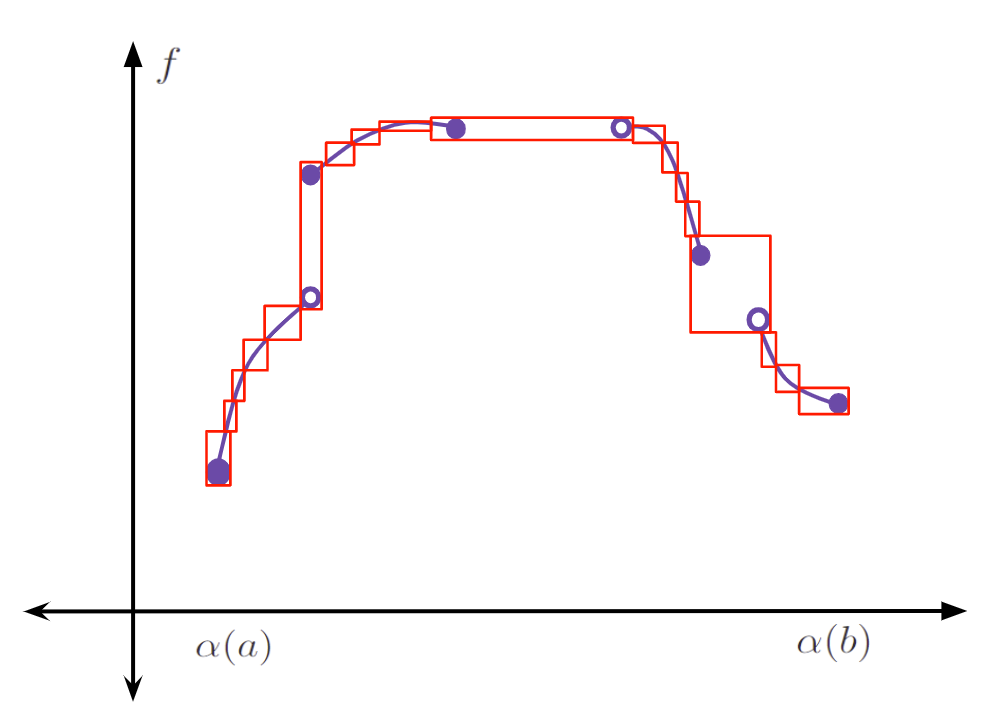
\includegraphics[scale=0.55]{Integrability_rectangles.png}
\end{center}

{\begin{myIndent}\exOne
   Imagine the above parametric graph of $(\alpha(t), f(t))$ for $t \in [a, b]$. An important\\ thing this diagram demonstrates is that both $f$ and $\alpha$ can be discontinuous.\retTwo

   Given some partition, each area surrounded by a red rectangle corresponds\\ to the quantity $(M_i - m_i)\Delta \alpha_i$. Also, the sum of all the areas in the red\\ rectangles is $U(P, f, \alpha) - L(P, f, \alpha)$. So by proposition 96, we know that\\ $f \in \mathscr{R}_a^b(\alpha)$ if and only if it possible to minimize the area inside those\\ rectangles.

   \newpage

   Observation:
   \begin{myIndent}\exTwo
      \begin{itemize}
         \item If $\alpha$ has a discontinuity at a point, then we are forced to have a wide\\ rectangle.
         \item If $f$ has a discontinuity at a point, then we are forced to have a tall\\ rectangle.
         \item If both $f$ and $\alpha$ are discontinuous at a point, then we're screwed\\ because we're stuck having a wide and tall rectangle.\retTwo\retTwo
      \end{itemize}
   \end{myIndent}

   \hTwo
   Proposition \propCount: If $f: [a, b] \longrightarrow \mathbb{R}$ is continuous and $\alpha: [a, b] \longrightarrow \mathbb{R}$ is\\ monotonically increasing, then $f \in \mathscr{R}_a^b(\alpha)$.
   
   {\begin{myIndent}\hThree
      Proof:\\
      Recalling proposition 96, let $\varepsilon > 0$. Since $f$ is continuous on the compact\\ set $[a, b]$, it is uniformly continuous. So, there is $\delta > 0$ such that:
      
      {\centering $\forall x, t, \in [a, b],\myHS |x-t|<\delta \Longrightarrow |f(x) - f(t)| < \frac{\varepsilon}{\alpha(b) - \alpha(a) + 1}$\\ [4pt]\par}

      {\begin{myDindent}\begin{myDindent}\teachComment
         We know that $\alpha(b) - \alpha(a) \geq 0$. So, we add $1$ to the\\ denominator to make sure the denominator can not\\ equal $0$.\retTwo
      \end{myDindent}\end{myDindent}}

      Now pick a partition $P = \{x_0, \ldots, x_n\}$ such that $\Delta x_i < \delta$ for all $i$. Then,\\ for each $i$ we have that $M_i - m_i \leq \frac{\varepsilon}{\alpha(b) - \alpha(a) + 1}$.\\ [-8pt]
      
      {\begin{myDindent}\begin{myDindent}\teachComment
         Technically, $M_i - m_i$ is strictly less than $\frac{\varepsilon}{\alpha(b) - \alpha(a) + 1}$\\ but we don't need that fact for this proof.\retTwo
      \end{myDindent}\end{myDindent}}

      Then:\\
      \begin{tabular}{l}
         $U(P, f, \alpha) - L(P, f, \alpha) = \sum\limits_{i=1}^n(M_i - m_i)\Delta \alpha_i$\\ [2pt]
         $\phantom{U(P, f, \alpha) - L(P, f, \alpha)} \leq \frac{\varepsilon}{\alpha(b) - \alpha(a) + 1}\sum\limits_{i=1}^n\Delta \alpha_i$\\ [2pt]
         $\phantom{U(P, f, \alpha) - L(P, f, \alpha)} =  \frac{\varepsilon}{\alpha(b) - \alpha(a) + 1}(\alpha(b) - \alpha(a)) \leq \varepsilon$.\retTwo\retTwo
      \end{tabular}
   \end{myIndent}}

   Proposition \propCount: If $f: [a, b] \longrightarrow \mathbb{R}$ is monotone and $\alpha: [a, b] \longrightarrow \mathbb{R}$ is\\ continuous and monotone increasing, then $f \in \mathscr{R}_a^b(\alpha)$.
   
   {\begin{myIndent}\hThree
      Proof:\\
      We'll assume that $f$ is monotonically increasing because the proof for if\\ $f$ is monotonically decreasing is mostly identical.\retTwo

      Let $\varepsilon > 0$ and pick $n \in \mathbb{Z}_+$ big enough that $\frac{\alpha(b) - \alpha(a)}{n}\left(f(b) - f(a)\right) < \varepsilon$.\\ Since $\alpha$ is continuous, by the intermediate value theorem we can find a\\ partition $P = \{x_0, \ldots, x_n\}$ with $x_0 = a$, $x_n = b$, and

      {\centering $\alpha(x_i) = \alpha(a) + \frac{i}{n}(\alpha(b) - \alpha(a))$.\par}

      \newpage

      Note then that $\Delta \alpha_i = \alpha(x_i) - \alpha(x_{i-1}) = \frac{\alpha(b)- \alpha(a)}{n}$ for all $i$. Also,\\ for all $i$ we have that $m_i = f(x_{i-1})$ and $M_i = f(x_i)$ because $f$ is\\ monotonically increasing. Hence:\\
      \begin{tabular}{l}
         $U(P, f, \alpha) - L(P, f, \alpha) = \sum\limits_{i=1}^n(M_i - m_i)\Delta \alpha_i$ \\ [4pt]
         $\phantom{U(P, f, \alpha) - L(P, f, \alpha)} = \frac{\alpha(b) - \alpha(a)}{n}\cdot \sum\limits_{i=1}^n(f(x_{i}) - f(x_{i-1}))$\\ [4pt]
         $\phantom{U(P, f, \alpha) - L(P, f, \alpha)} = \frac{\alpha(b) - \alpha(a)}{n}\left(f(b) - f(a)\right) < \varepsilon$\retTwo\retTwo
      \end{tabular}
   \end{myIndent}}

   Proposition \propCount: Suppose $f: [a, b] \longrightarrow \mathbb{R}$ is bounded and has only finitely\\ many discontinuities, and that $\alpha: [a, b] \longrightarrow \mathbb{R}$ is monotonically increasing and\\ continuous at every point where $f$ is discontinuous. Then $f \in \mathscr{R}_a^b(\alpha)$.
   
   {\begin{myIndent}\hThree
      Proof:\\
      Assume that $E = \{e_1, \ldots, e_m\}$ consists of all the points where $f$ is\\ discontinuous and define $M = \sup\{|f(x)| \mid a \leq x \leq b\}$. Let $\varepsilon > 0$.\\ Since $\alpha$ is continuous at each $e_j \in E$, we can pick numbers $u_j  < v_j$\\ for each $j \in \{1, \ldots, m\}$ such that:
      \begin{myIndent}\begin{enumerate}
            \item $e_j \in [u_j, v_j]$
            \item $e_j \in (u_j, v_j)$ when $e_j \notin \{a, b\}$
            \item $\sum\limits_{j=1}^m\left(\alpha(v_j) - \alpha(u_j)\right) < \varepsilon$\retTwo
      \end{enumerate}\end{myIndent}

      Now set $K = [a, b] \setminus \bigcup\limits_{j=1}^m(u_j, v_j)$.
      
      \retTwo

      Importantly, $K$ is a closed and bounded subset of $\mathbb{R}$, meaning it is\\ compact. Also, $f$ is continuous on $K$ because $K$ doesn't include any\\ points where $f$ is discontinuous except possibly $a$ and $b$. But then, if $f$\\ is discontinuous at $a$ or $b$, then $K$ includes $a$ or $b$ as an isolated point.\retTwo

      Therefore, $f$ is uniformly continuous on $K$, meaning there exists $\delta > 0$\\ such that $\forall s, t \in K, \myHS |s-t|<\delta \Longrightarrow |f(s) - f(t)| < \varepsilon$. So, pick any\\ partition $P = \{x_0, \ldots, x_n\}$ of $[a, b]$ such that:
      \begin{itemize}
         \item $\{u_1, v_1, u_2, v_2, \ldots, u_m, v_m\} \subseteq P \subseteq K$
         \item $x_{i-1} \notin \{u_1, u_2, \ldots, u_m\} \Longrightarrow \Delta x_i < \delta$ for all $i \in \{1, \ldots, n\}$\retTwo
      \end{itemize}

      Also define $M_i, m_i, \Delta \alpha_i$ as usual using $P$ and note that $M_i - m_i \leq 2M$.\\ Additionally because $P \subseteq K$, we know that $[x_{i-1}, x_{i}] \subseteq K$ unless\\ $x_{i-1} = u_j \text{ for some } j$. And if $x_{i-1} = u_j$, then $x_i = v_j$. Putting all of\\ this together, we get that:\\ [-8pt]

      {\center $(M_i - m_i)\Delta \alpha_i \leq \left\{ 
      \begin{matrix}
         2M(\alpha(v_j) - \alpha(u_j)) & \quad & \text{ if } x_{i-1} = u_j \text{ for some } j\\
         \varepsilon \Delta \alpha_i & \quad & \text{ if } x_{i-1} \notin \{u_1, \ldots, u_m\}
      \end{matrix} \right.$ \par}

      \newpage

      So:\\
      \begin{tabular}{l}
         $U(P, f, \alpha) - L(P, f, \alpha) = \sum\limits_{i=1}^n(M_i - m_i)\Delta \alpha_i$ \\ [4pt]
         $\phantom{U(P, f, \alpha) - L(P, f, \alpha)} \leq 2M \sum\limits_{j=1}^m\left(\alpha(v_j) - \alpha(u_j)\right) + \varepsilon(\alpha(b) - \alpha(a))$ \\ [7pt]
         $\phantom{U(P, f, \alpha) - L(P, f, \alpha)} < (2M + \alpha(b) - \alpha(a))\varepsilon$.\retTwo
      \end{tabular}

      $2M + \alpha(b) - \alpha(a)$ is a constant. Hence, it doesn't change the fact that\\ we can make $\varepsilon$ arbitrarily small and still find a partition $P$ such that\\ $U(P, f, \alpha) - L(P, f, \alpha) < \varepsilon$.\retTwo
   \end{myIndent}}
\end{myIndent}}

\markLecture{4/17/2024}


{\begin{myIndent}\hTwo
   Proposition \propCount: Suppose that $f: [a, b] \longrightarrow [m, M]$ such that $f \in \mathscr{R}_a^b(\alpha)$, and\\ that $\phi: [m, M] \longrightarrow \mathbb{R}$ is continuous. Then $\phi \circ f \in \mathscr{R}_a^b(\alpha)$.
   
   {\begin{myIndent}\hThree
      Proof:\\
      Since $\phi$ is continuous and $[m, M]$ is compact, $\phi$ is uniformly continuous.\\ So, there exists $\delta > 0$ such that $\delta < \varepsilon$ and:
      
      {\centering$\forall s, t \in [m, M],\myHS |s-t| < \delta \Longrightarrow |\phi(s) - \phi(t)| < \varepsilon$.\retTwo\par}

      Meanwhile, since $f \in \mathscr{R}_a^b(\alpha)$, we can pick a partition $P = \{x_0, \ldots, x_n\}$\\ of $[a, b]$ such that $U(P, f, \alpha) - L(P, f, \alpha) < \delta^2$. So, for each $i \in \{1, \ldots, n\}$,\\ define $m_i$ and $M_i$ using $P$ and $f$, as well as $m_i^*$ and $M_i^*$ using $P$ and $\phi \circ f$.\\ Then define $A = \{i \in \{1, \ldots n\} \mid M_i - m_i < \delta\}$ and $B = \{1, \ldots, n\} \setminus A$.\\ [-9pt]
      
      {\begin{myTindent}\begin{myIndent}\teachComment
         $A$ is our "good" set and $B$ is our "bad" set.
      \end{myIndent}\end{myTindent}}

      Now:
      
      \begin{tabular}{l}
         $\delta \sum\limits_{i \in B}\Delta \alpha_i \leq \sum\limits_{i \in B}(M_i - m_i)\Delta \alpha_i \leq \sum\limits_{i=1}^n(M_i - m_i)\Delta \alpha_i$\\ [4pt]
         $\phantom{\delta \sum\limits_{i \in B}\Delta \alpha_i \leq \sum\limits_{i \in B}(M_i - m_i)\Delta \alpha_i} = U(P, f, \alpha) - L(P, f, \alpha) < \delta^2$.\retTwo
      \end{tabular}

      So, $\sum\limits_{i \in B}\Delta \alpha_i < \delta$. At the same time, we have that $i \in A \Longrightarrow M_i^* - m_i^* \leq \varepsilon$.\retTwo Thus:\\ [-30pt]
      \begin{center}
         \begin{tabular}{l}
            $U(P, \phi \circ f, \alpha) - L(P, \phi \circ f, \alpha) = \sum\limits_{i=1}^n(M_i^* - m_i^*)\Delta \alpha_i$\\ [16pt]

            $\phantom{U(P, \phi \circ f, \alpha) - L(P, \phi \circ f, \alpha)} = \sum\limits_{i\in A}(M_i^* - m_i^*)\Delta \alpha_i + \sum\limits_{i\in B}(M_i^* - m_i^*)\Delta \alpha_i$\\ [14pt]

            $\phantom{U(P, \phi \circ f, \alpha) - L(P, \phi \circ f, \alpha)} \leq \varepsilon \sum\limits_{i\in A}\Delta \alpha_i  + 2\hspace{-0.5em}\sup\limits_{m\leq t\leq M}\hspace{-0.7em}|\phi(t)| \cdot \sum\limits_{i\in B} \Delta \alpha_i$\\ [14pt]

            $\phantom{U(P, \phi \circ f, \alpha) - L(P, \phi \circ f, \alpha)} \leq \varepsilon (\alpha(b) - \alpha(a))  + 2\delta \hspace{-0.5em}\sup\limits_{m\leq t\leq M}\hspace{-0.7em}|\phi(t)|$\\ [14pt]

            $\phantom{U(P, \phi \circ f, \alpha) - L(P, \phi \circ f, \alpha)} \leq (\alpha(b) - \alpha(a) + 2\hspace{-0.5em}\sup\limits_{m\leq t\leq M}\hspace{-0.7em}|\phi(t)|)\varepsilon$
         \end{tabular}
      \end{center}

      \newpage

      Now $\alpha(b) - \alpha(a) + 2\hspace{-0.5em}\sup\limits_{m\leq t\leq M}\hspace{-0.7em}|\phi(t)|$ is a constant.\retTwo
      
      Thus, we've still shown that we can can make $\varepsilon$ arbitrarily small and then\\ find a partition $P$ such that $U(P, f, \alpha) - L(P, f, \alpha) < \varepsilon$.\retTwo
   \end{myIndent}}
\end{myIndent}}

\mySepTwo

Next, we explore the properties of integrals\ldots\retTwo

{\begin{myIndent}\hTwo
   Proposition \propCount: Suppose that $c \in \mathbb{R}$, that $f, f_1, f_2 : [a, b] \longrightarrow \mathbb{R}$ are bounded,\\ and that $\alpha, \alpha_1, \alpha_2: [a, b] \longrightarrow \mathbb{R}$ be monotone increasing.
   
   \begin{enumerate}
      \item[(A)] {\fontsize{12.5}{14.5}\selectfont$\underline{\int_a^b}f_1d\alpha + \underline{\int_a^b}f_2d\alpha \leq \underline{\int_a^b}(f_1 + f_2)d\alpha$} \hspace{0.2em}and\hspace{0.2em} {\fontsize{12.5}{14.5}\selectfont$\overline{\int_a^b}f_1d\alpha + \overline{\int_a^b}f_2d\alpha \geq \overline{\int_a^b}(f_1 + f_2)d\alpha$}\\
      Hence, $f_1, f_2 \in \mathscr{R}_a^b(\alpha) \Longrightarrow (f_1 + f_2) \in \mathscr{R}_a^b(\alpha)$ with:
      
      {\centering$\int_a^bf_1d\alpha + \int_a^bf_2d\alpha = \int_a^b(f_1 + f_2)d\alpha$.\retTwo\par}

      {\begin{myIndent}\hThree
         This follows from the fact that:
         \begin{myIndent}
            \begin{itemize}
               \item $\hspace{-1.2em}\inf\limits_{x_{i-1}\vphantom{\int^b} \leq x \leq x_i}\hspace{-1.1em}f_1(x) + \hspace{-1.1em}\inf\limits_{x_{i-1} \leq\vphantom{\int^b} x \leq x_i}\hspace{-1.1em}f_2(x) \leq \hspace{-1em}\inf\limits_{x_{i-1} \leq x\vphantom{\int^b} \leq x_i}\hspace{-1em}(f_1(x) + f_2(x))$\\
               
               \item $\hspace{-1.2em}\sup\limits_{x_{i-1} \leq x \leq x_i}\hspace{-1em}f_1(x) + \hspace{-1em}\sup\limits_{x_{i-1} \leq x \leq x_i}\hspace{-1.1em}f_2(x) \geq \hspace{-1em}\sup\limits_{x_{i-1} \leq x \leq x_i}\hspace{-1em}(f_1(x) + f_2(x))$\\
            \end{itemize}
            
            \begin{myDindent}\hFour
               We proved this last quarter in a homework assignment.\\ Intuitively though, this is because  $f_1$ and $f_2$ might reach\\ their most extreme values at different points, and in that\\ case you can't maximize or minimize two functions at\\ the same time.\retTwo
            \end{myDindent}
         \end{myIndent}
      \end{myIndent}}

      Also, if $c \geq 0$, then $\underline{\int_a^b}cfd\alpha = c\underline{\int_a^b}fd\alpha$ and $\overline{\int_a^b}cfd\alpha = c\overline{\int_a^b}fd\alpha$. Meanwhile,\\ [-4pt] if $c \leq 0$, then $\underline{\int_a^b}cfd\alpha = c\overline{\int_a^b}fd\alpha$ and $\overline{\int_a^b}cfd\alpha = c\underline{\int_a^b}fd\alpha$. Hence, we have\\ [2pt] that if $f \in \mathscr{R}_a^b(\alpha)$, then:

      {\centering $\int_a^bcfd\alpha = c\int_a^bfd\alpha$. \retTwo\par}

      {\begin{myIndent}\hThree
         This similarly follows from the fact that:
         \begin{myIndent}
            \begin{itemize}
               \item when $c \geq 0$:
               
               \begin{tabular}{c c c}
                  $\circ\hspace{-1.2em}\inf\limits_{x_{i-1}\vphantom{\int^b} \leq x \leq x_i}\hspace{-1em}(cf(x)) = c\hspace{-1.22em}\inf\limits_{x_{i-1} \leq\vphantom{\int^b} x \leq x_i}\hspace{-1.15em}f(x)$ & $\phantom{a}$ &

                  $\circ\hspace{-0.9em}\sup\limits_{x_{i-1} \leq x \leq x_i}\hspace{-1em}(cf(x)) = c\hspace{-1em}\sup\limits_{x_{i-1} \leq x \leq x_i}\hspace{-1em}f(x)$
               \end{tabular}\\

               \item when $c \leq 0$:
               
               \begin{tabular}{c c c}
                  $\circ\hspace{-1.2em}\inf\limits_{x_{i-1}\vphantom{\int^b} \leq x \leq x_i}\hspace{-1em}(cf(x)) = c\hspace{-1.0em}\sup\limits_{x_{i-1} \leq x \leq x_i}\hspace{-1em}f(x)$ & $\phantom{a}$ &

                  $\circ\hspace{-0.9em}\sup\limits_{x_{i-1} \leq x \leq x_i}\hspace{-1em}(cf(x)) = c\hspace{-1.1em}\inf\limits_{x_{i-1}\vphantom{\int^a} \leq x \leq x_i}\hspace{-1.2em}f(x)$\retTwo
               \end{tabular}
            \end{itemize}

            \begin{myDindent}\hFour
               This is another past homework question.
            \end{myDindent}
         \end{myIndent}
      \end{myIndent}}

      \newpage

      \item[(B)] {\fontsize{12}{14}\selectfont$\left(\vphantom{\int^b}\forall x \in [a, b], \myHS f_1(x) \leq f_2(x)\right) \Longrightarrow \underline{\int_a^b}f_1d\alpha \leq \underline{\int_a^b}f_2d\alpha$ and $\overline{\int_a^b}f_1d\alpha \leq \overline{\int_a^b}f_2d\alpha$}.\\ [-11pt]
      
      {\begin{myIndent}\hThree
         This is immediate from our definitions.
         \retTwo
      \end{myIndent}}

      \item[(C)] If $c \in (a, b)$, then {\fontsize{12}{14}\selectfont$\underline{\int_a^b}fd\alpha = \underline{\int_a^c}fd\alpha + \underline{\int_c^b}fd\alpha$ and $\overline{\int_a^b}fd\alpha = \overline{\int_a^c}fd\alpha + \overline{\int_c^b}fd\alpha$.}
      
      {\begin{myIndent}\hThree
         Proof:\\
         We'll focus on the lower integral statement since the proof for the\\ upper integral statement is mostly identical.\retTwo

         By proposition 94, we have that:
         
         {\centering$\underline{\int_a^b}fd\alpha = \hspace{-0.2em}\sup\limits_{P \in \mathcal{P}_{a,b}}\hspace{-0.4em}L(P, f, \alpha) = \hspace{-0.2em}\sup\limits_{P \in \mathcal{P}_{a,b}}\hspace{-0.4em}L(P \cup \{c\}, f, \alpha)$.\retTwo\par}

         Next, setting $P_1 = \left(P \cup \{c\}\right) \cap [a, c]$ and $P_2 = \left(P \cup \{c\}\right) \cap [c, b]$, we\\ have that:

         {\centering
         \begin{tabular}{l}
            $\sup\limits_{P \in \mathcal{P}_{a,b}}\hspace{-0.4em}L(P \cup \{c\}, f, \alpha) = \hspace{-0.2em}\sup\limits_{
            \begin{smallmatrix}
               P_1 \in \mathcal{P}_{a,c}\\
               P_2 \in \mathcal{P}_{c,b}
            \end{smallmatrix}}\hspace{-0.4em}\left(L(P_1, f, \alpha) + \hspace{-0.2em}\sup\limits_{P_2 \in \mathcal{P}_{c,b}}\hspace{-0.4em}L(P_2, f, \alpha)\right)$\\ [32pt]

            $\phantom{\sup\limits_{P \in \mathcal{P}_{a,b}}\hspace{-0.4em}L(P \cup \{c\}, f, \alpha)} = \hspace{-0.2em}\sup\limits_{P_1 \in \mathcal{P}_{a,c}}\hspace{-0.4em}L(P_1, f, \alpha) + \hspace{-0.2em}\sup\limits_{P_2 \in \mathcal{P}_{c,b}}\hspace{-0.4em}L(P_2, f, \alpha)$\\ [16pt]

            $\phantom{\sup\limits_{P \in \mathcal{P}_{a,b}}\hspace{-0.4em}L(P \cup \{c\}, f, \alpha)} = \underline{\int_a^c}fd\alpha + \underline{\int_c^b}fd\alpha$\retTwo
         \end{tabular}\retTwo\par}
      \end{myIndent}}

      \item[(D)] $\left|\underline{\int_a^b}fd\alpha\right|, \left|\overline{\int_a^b}fd\alpha\right| \leq (\alpha(b) - \alpha(a))\cdot \sup\limits_{a\leq x \leq b}|f(x)|$.
      
      {\begin{myIndent}\hThree
         This is immediate from our definitions.
         \retTwo
      \end{myIndent}}

      \item[(E)] {\fontsize{12}{14}\selectfont$\underline{\int_a^b}fd(\alpha_1 + \alpha_2) = \underline{\int_a^b}fd\alpha_1 + \underline{\int_a^b}fd\alpha_2$ and $\overline{\int_a^b}fd(\alpha_1 + \alpha_2) = \overline{\int_a^b}fd\alpha_1 + \overline{\int_a^b}fd\alpha_2$}\\ 
      Also, if $c \geq 0$, then $\underline{\int_a^b}cfd\alpha = c\underline{\int_a^b}fd\alpha$ and $\overline{\int_a^b}cfd\alpha = c\overline{\int_a^b}fd\alpha$.\\ [-6pt]
      
      \begin{myIndent}\hThree
         This immediately follows from the fact that\\ $\Delta(\alpha_1 + \alpha_2)_i = \Delta(\alpha_1)_i + \Delta(\alpha_2)_i$ and $\Delta(c\alpha)_i = c\cdot\Delta\alpha_i$.
      \end{myIndent}
   \end{enumerate}
\end{myIndent}}

\markLecture{4/19/2024}

{\begin{myIndent}\hTwo
   Proposition \propCount: If $f, g \in \mathscr{R}_a^b(\alpha)$, then:
   \begin{enumerate}
      \item[(A)] $fg \in \mathscr{R}_a^b(\alpha)$.\\[-6pt]
      {\begin{myIndent}\hThree
         Proof:\\
         By propositions 101 and 102, we know that $(f + g)^2 \in \mathscr{R}_a^b(\alpha)$ and\\ $(f - g)^2 \in \mathscr{R}_a^b(\alpha)$.   Therefore {\fontsize{12.8}{14.8}\selectfont$fg = \frac{1}{4}\left((f+g)^2 + (f-g)^2\right) \in \mathscr{R}_a^b(\alpha)$}.
      \end{myIndent}}
      
      \newpage

      \item[(B)] $|f| \in \mathscr{R}_a^b(\alpha)$ and $\left|\int_a^b fd\alpha\right| \leq \int_a^b |f|d\alpha$.\\ [-6pt]
      
      {\begin{myIndent}\hThree
         Proof:\\
         We know that $|f| \in \mathscr{R}_a^b(\alpha)$ by proposition 101. Then, because\\ $f(x), -f(x) \leq |f(x)|$ for all $x \in [a, b]$, we know by proposition\\ 102.B that $\int_a^bfd\alpha \leq \int_a^b|f|d\alpha$ and $-\int_a^bfd\alpha \leq \int_a^b|f|d\alpha$. Therefore:
         
         {\centering$\left|\int_a^b fd\alpha\right| \leq \int_a^b |f|d\alpha$.\retTwo\retTwo\par}
      \end{myIndent}}
   \end{enumerate}
\end{myIndent}}

The \udefine{unit step function} $I$ is defined by: $I(x) = \left\{
\begin{matrix}
   0 & \text{ when } x \leq 0 \\
   1 & \text{ when } x > 1
\end{matrix}\right.$\retTwo

{\begin{myIndent}\hTwo
   Proposition \propCount: Suppose $s \in [a, b)$ and $f: [a, b] \longrightarrow \mathbb{R}$ be bounded. If\\ $\alpha(x) = I(x - s)$, we have that $f \in \mathscr{R}_a^b(\alpha)$ if and only if $f(s+) = f(s)$.\\ Furthermore, $\int_a^bfd\alpha = f(s)$.\\ [-6pt]

   {\begin{myIndent}\hThree
      Proof:\\
      Letting $P = \{x_0, \ldots, x_n\}$ be any partition of $[a, b]$, we can assume because\\ of proposition 94 that $s \in P$. So let $j$ be such that $x_j = s$. Then note that\\ $L(P, f, \alpha) = m_{j+1} = \hspace{-1.05em}\inf\limits_{x_j \leq x \vphantom{\int^a}\leq x_{j+1}}\hspace{-1.1em}f(x)$ and $U(P, f, \alpha) = M_{j+1} = \hspace{-1.05em}\sup\limits_{x_j \leq x \leq x_{j+1}}\hspace{-1.1em}f(x)$.\retTwo

      ($\Longrightarrow$) If $f \in \mathscr{R}_a^b$, then for all $\varepsilon > 0$, there exists a partition $P$ such that\\ $U(P, f, \alpha) - L(P, f, \alpha) < \varepsilon$. Then because $f(x), f(t) \in [m_{j+1}, M_{j+1}]$\\ for all $t \in [x_j, x_{j+1}]$, by setting $\delta = x_{j+1} - x_j$ we know that:
      
      {\centering$t \in [s, s + \delta] \Longrightarrow |f(t) - f(s)| \leq M_{j+1} - m_{j+1} < \varepsilon$.\retTwo\par}

      So $f(s+) = f(s)$.\retTwo

      ($\Longleftarrow$) Meanwhile if $f(s+) = f(s)$, then for any $\varepsilon > 0$ there exists $\delta > 0$\\ such that $t \in [s, s + \delta] \Longrightarrow |f(t) - f(s)| < \sfrac{\varepsilon}{2}$. So, let $P = \{x_0, \ldots, x_n\}$\\ be a partition of $[a, b]$ such that $x_j = s$ and $x_{j+1} = s + \delta$. Then\\ $m_{j+1} \geq f(s) - \sfrac{\varepsilon}{2}$ and $M_{j+1} \leq f(s) + \sfrac{\varepsilon}{2}$. Hence:

      {\centering $U(P, f, \alpha) - L(P, f, \alpha) = M_{j+1} - m_{j+1} < \varepsilon$ \retTwo\par}

      This means that $f \in \mathscr{R}_a^b(\alpha)$.\retTwo

      Finally, note that for all $\varepsilon > 0$ there exists a partition $P$ such that\\ $U(P, f, \alpha) = M_{j+1} < f(s) + \varepsilon$ and $L(P, f, \alpha) = m_{j+1} > f(s) + \varepsilon$.\\ Thus:

      {\centering $\underline{\int_a^b}fd\alpha = \overline{\int_a^b}fd\alpha = \int_a^bfd\alpha = f(s)$.\retTwo\par}
   \end{myIndent}}

   \newpage

   Proposition \propCount: Let $(c_n)$ be a sequence of non-negative reals with $\sum c_n < \infty$.\\ Also let $(s_n)$ be a sequence in $[a, b)$ and set $\alpha(x) = \sum\limits_{n=1}^\infty c_nI(x - s_n)$.

   {\begin{myTindent}\begin{myDindent}\hFour
      Interestingly, this is the same function we made\\ at the bottom of page 63 during math 140A.\retTwo
   \end{myDindent}\end{myTindent}}

   If $f: [a, b] \longrightarrow \mathbb{R}$ is continuous, then $f \in \mathscr{R}_a^b(\alpha)$  and $\int_a^bfd\alpha = \sum\limits_{n=1}^\infty c_nf(s_n)$.\\ [ -6pt]

   
   {\begin{myIndent}\hThree
      Proof:\\
      Note that $\alpha(x)$ converges absolutely by comparison with $(c_n)$ for all\\ [1pt] $x \in [a, b]$. Also, $\alpha$ is monotonically increasing with $\alpha(b) = \sum c_n$.\retTwo

      Now let $\varepsilon > 0$ and pick $N$ with $\hspace{-0.65em}\sum\limits_{n = N+1}^\infty\hspace{-0.7em} c_n < \varepsilon$. Also set $M = \hspace{-0.3em}\sup\limits_{a\leq x\leq b}\hspace{-0.3em}|f(x)|$\retTwo
      
      By proposition 98, we know that $f \in \mathscr{R}_a^b(\alpha)$. So finally, define\\
      $\beta(x) = \sum\limits_{i=1}^N c_k I(x - s_k)$ and $\gamma(x) = \hspace{-0.65em}\sum\limits_{i=N+1}^\infty\hspace{-0.65em} c_k I(x - s_k)$. Then\\ $\gamma = \alpha - \beta$ and $f \in \mathscr{R}_a^b(\beta), \mathscr{R}_a^b(\gamma)$. So:\\
      
      \begin{center}{\fontsize{12}{14}\selectfont
         \begin{tabular}{l}
            $\left|\cyPen{\sum\limits_{k=1}^n c_kf(s_k)}\vphantom{.} - \int_a^b fd\alpha\right| = \left| \cyPen{\int_a^b fd\beta}\vphantom{.} - \int_a^b fd\alpha \right|$\\ [8pt]
            
            $\phantom{\left|\cyPen{\sum\limits_{k=1}^n c_kf(s_k)}\vphantom{.} - \int_a^b fd\alpha\right|} = \left|\int_a^b fd(\beta - \alpha)\right|$\\ [8pt]

            $\phantom{\left|\cyPen{\sum\limits_{k=1}^n c_kf(s_k)}\vphantom{.} - \int_a^b fd\alpha\right|} = \left|\int_a^b fd\gamma\right| \leq \int_a^b|f|d\gamma$\\ [4pt]

            $\phantom{\left|\cyPen{\sum\limits_{k=1}^n c_kf(s_k)}\vphantom{.} - \int_a^b fd\alpha\right| = \left|\int_a^b fd\gamma\right|} \leq \int_a^bMd\gamma = M(\gamma(b) - \gamma(a))$\\ [4pt]

            $\phantom{\left|\cyPen{\sum\limits_{k=1}^n c_kf(s_k)}\vphantom{.} - \int_a^b fd\alpha\right| = \left|\int_a^b fd\gamma\right| \leq \int_a^bMd\gamma} = M\left(\hspace{0em}\sum\limits_{i=N+1}^\infty\hspace{-0.5em} c_k - 0\right) < M\varepsilon$
         \end{tabular}}
      \end{center}

      As $\varepsilon$ is arbitrary, we thus have that $\int_a^bfd\alpha = \sum\limits_{n=1}^\infty c_nf(s_n)$.\\ [-4pt]
      
      
      {\begin{myTindent}\teachComment
         Note, we assumed $(c_n)$ and $(s_n)$ are infinite sequences\\ because if $(c_n)$ and $(s_n)$ have finitely many elements, then\\ this theorem holds trivially because of proposition 102.
      \end{myTindent}}
      \retTwo
   \end{myIndent}}

   Proposition \propCount: Let $\alpha: [a, b] \longrightarrow \mathbb{R}$ be monotonically increasing and\\ differentiable, and assume $\alpha^\prime \in \mathscr{R}_a^b$. Also let $f: [a, b] \longrightarrow \mathbb{R}$ be bounded.\\ Then $f \in \mathscr{R}_a^b(\alpha) \Longleftrightarrow f\alpha^\prime \in \mathscr{R}_a^b$ with $\int_a^bfd\alpha = \int_a^bf\alpha^\prime dx$.\\ [-6pt]
   
   \begin{myIndent}\hThree
      Proof:\\
      It suffices to show $\underline{\int_a^b}fd\alpha = \underline{\int_a^b}f\alpha^\prime dx$ and $\overline{\int_a^b}fd\alpha = \overline{\int_a^b}f\alpha^\prime dx$.

      \newpage

      We'll focus on proving the lower integral statement because the proof for\\ the upper integral statement is mostly identical. Set $M = \hspace{-0.1em}\sup\limits_{a \leq x \leq b}\hspace{-0.2em}|f(x)|$\\ [-8.5pt] and let $\varepsilon > 0$.\retTwo

      Pick partitions $P_1, P_2, P_3$ such that:
      \begin{itemize}
         \item $L(P_1, f, \alpha) > \underline{\int_a^b}fd\alpha - \varepsilon$
         \item $L(P_2, f\alpha^\prime) > \underline{\int_a^b}f\alpha^\prime dx - \varepsilon$\\ [-10pt]
         \item $U(P_3, \alpha^\prime) - L(P_3, \alpha^\prime) < \varepsilon$\retTwo
      \end{itemize}

      Then set $P = P_1 \cup P_2 \cup P_3 = \{x_0, \ldots, x_n\}$ so that $P$ satisfies all of\\ the above inequalities.\retTwo
      
      By the mean value theorem, we know there exists $t_i \in [x_{i-1}, x_i]$ with\\ $\Delta \alpha_i = \alpha^\prime(t_i)\Delta x_i$ for each $1 \leq i \leq n$. Also, given any  $s_i \in [x_{i-1}, x_i]$\\ for each $1 \leq i \leq n$, we know by proposition 97.B and because\\ $U(P, \alpha^\prime) - L(P, \alpha^\prime) < \varepsilon$ that:

      {\centering $\sum\limits_{i=1}^n|f(s_i) - f(t_i)|\Delta x_i < \varepsilon$. \retTwo\par}

      Therefore:

      \begin{center}
         {\fontsize{11.5}{13.5}\selectfont\begin{tabular}{l}
            $\left|\sum\limits_{i=1}^n\left( f(s_i)\Delta\alpha_i - f(s_i)\alpha^\prime(s_i)\Delta x_i\right)\right| = \left|\sum\limits_{i=1}^n\left( f(s_i)\alpha^\prime(t_i)\Delta x_i -f(s_i)\alpha^\prime(s_i)\Delta x_i\right)\right|$\\ [12pt]

            $\phantom{\left|\sum\limits_{i=1}^n\left( f(s_i)\Delta\alpha_i - f(s_i)\alpha^\prime(s_i)\Delta x_i\right)\right|} \leq M \cdot \left|\sum\limits_{i=1}^n \alpha^\prime(t_i)\Delta x_i - \sum\limits_{i=1}^n \alpha^\prime(s_i)\Delta x_i\right| < M\varepsilon$\\ [4pt]
         \end{tabular}}\retTwo
      \end{center}

      Hence, letting $s_i = \hspace{-1.2em}\inf\limits_{x_{i-1}\leq\vphantom{\int^a} x \leq x_i}\hspace{-1.15em}f(x)$ for each $1 \leq i \leq n$,we have that:

      \begin{center}
         {\fontsize{11.4}{13.4}\selectfont\begin{tabular}{l}
            $\underline{\int_a^b}fd\alpha \geq L(P, f, \alpha) = \sum\limits_{i=1}^nf(s_i)\Delta\alpha_i > \sum\limits_{i=1}^nf(s_i)\alpha^\prime(s_i)\Delta x_i - M\varepsilon$\\ [8pt]

            $\phantom{\underline{\int_a^b}fd\alpha \geq L(P, f, \alpha) = \sum\limits_{i=1}^nf(s_i)\Delta\alpha_i} = L(P, f\alpha^\prime) - M\varepsilon > \overline{\int_a^b}f\alpha^\prime dx - (M + 1)\varepsilon$
         \end{tabular}}\retTwo
      \end{center}

      Similarly, letting $s_i = \hspace{-1.2em}\inf\limits_{x_{i-1}\leq\vphantom{\int^a} x \leq x_i}\hspace{-1.15em}f(x)\alpha^\prime(x)$ for each $1 \leq i \leq n$,we have that:

      \begin{center}
         {\fontsize{11.4}{13.4}\selectfont\begin{tabular}{l}
            $\underline{\int_a^b}f\alpha^\prime dx \geq L(P, f\alpha^\prime) = \sum\limits_{i=1}^nf(s_i)\alpha^\prime(s_i)\Delta x_i > \sum\limits_{i=1}^nf(s_i)\Delta\alpha_i - M\varepsilon$\\ [6pt]

            $\phantom{\underline{\int_a^b}f\alpha^\prime dx \geq L(P, f\alpha^\prime) = \sum\limits_{i=1}^nf(s_i)a\alpha^\prime(s_i)\Delta_i} = L(P, f, \alpha) - M\varepsilon$\\ [-4pt]

            $\phantom{\underline{\int_a^b}f\alpha^\prime dx \geq L(P, f\alpha^\prime) = \sum\limits_{i=1}^nf(s_i)a\alpha^\prime(s_i)\Delta_i} > \overline{\int_a^b}f\alpha^\prime dx - (M + 1)\varepsilon$
         \end{tabular}}\retTwo
      \end{center}

      Since $\varepsilon > 0$ was arbitrary, we conclude that $\underline{\int_a^b}fd\alpha = \underline{\int_a^b}f\alpha^\prime dx$.
   \end{myIndent}
\end{myIndent}}

\newpage

\markLecture{4/22/2024}

{\begin{myIndent}\hTwo
   Proposition \propCount: Let $\alpha: [a, b] \longrightarrow \mathbb{R}$ be monotone increasing and let\\ $f: [a, b] \longrightarrow \mathbb{R}$ with $f \in \mathscr{R}_a^b(\alpha)$. If $\phi: [A, B] \longrightarrow [a, b]$ is a strictly\\ increasing continuous bijection, then $\int_A^B \left(f\circ\phi\right) d(\alpha \circ \phi) = \int_a^b fd\alpha$.\\ [-6pt]

   {\begin{myIndent}\hThree
      Proof:\\
      Note that $\phi$ produces a bijection between partitions of $[A, B]$ and\\ partitions of $[a, b]$. It sends the partition $Q = \{y_0, \ldots, y_n\}$ of $[A, B]$ to\\ $P = \phi(Q) = \{x_0, \ldots, x_n\}$ where $x_i = \phi(y_i)$ for all $1 \leq i \leq n$.\retTwo

      With this notation, we have that:
      
      {\centering $\hspace{-1.05em}\inf\limits_{y_{j-1} \vphantom{\int_b}\leq t \leq y_{j}}\hspace{-1.1em}f\circ \phi(t) = \hspace{-1.05em}\inf\limits_{x_{j-1} \vphantom{\int_b}\leq t \leq x_{j}}\hspace{-1.1em}f(t)$ and $\hspace{-1.05em}\sup\limits_{y_{j-1}\leq t \leq y_{j}}\hspace{-0.9em}f\circ \phi(t) = \hspace{-1.05em}\sup\limits_{x_{j-1} \leq t \leq x_{j}}\hspace{-1em}f(t)$.\retTwo\par}

      Also, $\Delta(\alpha \circ \phi)_i = \Delta\alpha_i$. So $U(Q, f\circ \phi, \alpha \circ \phi) = U(P, f, \alpha)$ and\\ $L(Q, f\circ \phi, \alpha \circ \phi) = L(P, f, \alpha)$. Hence, the theorem above\\ follows from taking the $\sup$ and $\inf$ over all $Q$.\retTwo
      
      {\begin{myTindent}\teachComment
         Note: if $\alpha(x) = x$ and $\phi$ is differentiable with $\phi^\prime \in \mathscr{R}_a^b$,\\ then using the previous theorem we have that:

         {\centering $\int_a^bf(x)dx = \int_A^B(f \circ \phi)d\phi = \int_A^B f(\phi(x))\phi^\prime(x)dx$ \retTwo\par}
      \end{myTindent}}
   \end{myIndent}}

   Proposition \propCount: (part 1 of the fundamental theorem of calculus):\\
   Let $f \in \mathscr{R}_a^b$ and define $F(x) = \int_a^xf(t)dt$ on the domain $[a, b]$. Then:
   \begin{enumerate}
      \item $F$ is continuous.
      
      {\begin{myIndent}\hThree
         Proof:\\
         Let $\varepsilon > 0$ and set $M > 0$ such that $M \geq |f(x)|$ for all $x \in [a, b]$.\\ Then set $\delta < \sfrac{\varepsilon}{M}$ and consider any $a \leq x \leq y \leq b$ with $|x - y| < \delta$.\retTwo

         By proposition 102, we know that:
         
         {\centering$|F(y) - F(x)| = |\int_x^yf(t)dt| \leq M|y-x| < M\delta < \varepsilon$.
         \retTwo\par}

         So, $F$ is uniformly continuous.
         \retTwo
      \end{myIndent}}

      \item If $f$ is continuous at $x_0$, then $F$ is differentiable at $x_0$ and $F^\prime(x_0) = f(x_0)$.
      
      {\begin{myIndent}\hThree
         Proof:\\
         Let $\varepsilon > 0$ and pick $\delta > 0$ such that for all $t \in [a, b], \myHS |t - x_0| < \delta$\\ implies that  $|f(t) - f(x_0)| < \varepsilon$. Then consider any $s \neq x_0$ such\\ that $s \in [a, b]$ and $|s - x_0| < \delta$.\retTwo

         Notice that $f(x_0) = \frac{1}{|s - x_0|}{\displaystyle\int_{\text{\footnotesize $\min(s, x_0)$}}^{\text{\footnotesize $\max(s, x_0)$}}}{\hspace{-3em} f(x_0)dt}$.

         \newpage

         Therefore,
         \begin{center}
            \begin{tabular}{l}
               $\left|\frac{F(s) - F(x_0)}{s - x_0} - f(x_0)\right| = \frac{1}{|s - x_0|}\left|{\displaystyle\int_{\text{\footnotesize $\min(s, x_0)$}}^{\text{\footnotesize $\max(s, x_0)$}}}{\hspace{-3em} \left(f(t) - f(x_0)\right)dt}\right|$\\ [20pt]

               $\phantom{\left|\frac{F(s) - f(x_0)}{s - x_0} - f(x_0)\right|} \leq \frac{1}{|s - x_0|}{\displaystyle\int_{\text{\footnotesize $\min(s, x_0)$}}^{\text{\footnotesize $\max(s, x_0)$}}}{\hspace{-3em} \left|f(t) - f(x_0)\right|dt}$\\ [20pt]

               $\phantom{\left|\frac{F(s) - f(x_0)}{s - x_0} - f(x_0)\right|} < {\frac{1}{|s - x_0|}{\displaystyle\int_{\text{\footnotesize $\min(s, x_0)$}}^{\text{\footnotesize $\max(s, x_0)$}}}{\hspace{-3em} \varepsilon dt}} \hspace{1.4em} = \frac{1}{|s - x_0|}|s - x_0|\varepsilon = \varepsilon$
            \end{tabular}\retTwo
         \end{center}

         So $\lim\limits_{s \rightarrow x_0}\left|\frac{f(s) - F(x_0)}{s - x_0} - f(x_0)\right| = 0$, meaning that $F^\prime(x_0) = f(x_0)$.
         \retTwo\retTwo
      \end{myIndent}}
   \end{enumerate}

   Proposition \propCount: (part 2 of the fundamental theorem of calculus)\\
   If $f \in \mathscr{R}_a^b$ and there is a differentiable function $F: [a, b] \longrightarrow \mathbb{R}$ with $F^\prime = f$,\\ then $\int_a^b fdx = F(b) - F(a)$.\\ [-6pt]
   
   {\begin{myIndent}\hThree
      Proof:\\
      Let $\varepsilon > 0$. Since $f \in \mathscr{R}_a^b$, there is a partition $P = \{x_0, \ldots, x_n\}$ of $[a, b]$\\ with $U(P, f) - L(P, f) < \varepsilon$.\retTwo

      Now, by the mean value theorem, for each $1 \leq i \leq n$ pick $t_i \in [x_{i-1}, x_i]$\\ such that $F(x_i) - F(x_{i-1}) = F^\prime(t_i)\Delta x_i = f(t_i)\Delta x_i$.\retTwo
      
      Then $F(b) - F(a) = \sum\limits_{i=1}^n f(t_i)\Delta x_i$ and $\sum\limits_{i=1}^n f(t_i)\Delta x_i$ is within $\varepsilon$ of $\int_a^bfdx$\\ [-6pt] by proposition 97.C.\retTwo\retTwo
   \end{myIndent}}

   Proposition \propCount: (integration by parts)\\
   If $F^\prime = f \in \mathscr{R}_a^b$ and $G^\prime = g \in \mathscr{R}_a^b$, then $Fg, fG \in \mathscr{R}_a^b$ with:
   
   {\centering $ \int_a^b Fgdx = F(b)G(b) - F(a)G(a) - \int_a^b fGdx $ \retTwo\par}
   
   {\begin{myIndent}\hThree
      Proof:\\
      Since $F$ and $G$ are differentiable, they are continuous. Hence $F, G \in \mathscr{R}_a^b$.\\ In turn, this means by proposition 103 that $Fg, fG \in \mathscr{R}_a^b$. So now, apply\\ the fundamental theorem of calculus to $H(x) = F(x)G(x)$ and its\\ derivative:
      
      \begin{center}{\fontsize{12.5}{14.5}\selectfont
         \begin{tabular}{c}
            $\int_a^b H^\prime dx = \int_a^b (Fg + fG)dx = F(b)G(b) - F(a)G(a) = H(b) - H(a)$
         \end{tabular}}
      \end{center}
   \end{myIndent}}

\end{myIndent}}

% ~~~~~~~~~~~~~~~~~~~~~~~~~~~~~~~~~~~~~~~~~~~~~~~~~~~~~~~~~~~~~~~~~~~~~~ %
\newpage
{\huge \color{Black} \textbf{A List of How The Proposition Numbering in my Notes Lines up With Our Textbook:} \retTwo}
\exOne

\begin{allowTableDashes}
   \begin{tabular}{ c|c||c|c }
      Proposition Number & Label in Textbook & Proposition Number & Label in Textbook \\ \hline
      
      \myVS 83 & 5.2 & 84 & 5.3 \\ \hdashline[10pt/3pt]
      \myVS 85 & 5.5 & 86 & 5.8 \\ \hdashline[10pt/3pt]
      \myVS 87 & 5.9  & 88 & 5.10 \\ \hdashline[10pt/3pt]
      \myVS 89 & 5.11 & 90 & 5.12 \\ \hdashline[10pt/3pt]
      \myVS 91 & 5.13 & 92 & 5.15 \\ \hdashline[10pt/3pt]
      \myVS 93 & 5.19 & 94 & 6.4  \\ \hdashline[10pt/3pt]
      \myVS 95 & 6.5 & 96 & 6.6 \\ \hdashline[10pt/3pt]
      \myVS 97 & 6.7 & 98 & 6.8 \\ \hdashline[10pt/3pt]
      \myVS 99 & 6.9 & 100 & 6.10 \\ \hdashline[10pt/3pt]
      \myVS 101 & 6.11 & 102 & 6.12 \\ \hdashline[10pt/3pt]
      \myVS 103 & 6.13 & 104 & 6.15 \\ \hdashline[10pt/3pt]
      \myVS 105 & 6.16 & 106 & 6.17 \\ \hdashline[10pt/3pt]
      \myVS 107 & 6.19 & 108 & 6.20 \\ \hdashline[10pt/3pt]
      \myVS 109 & 6.21 & 110 & 6.22 \\ \hdashline[10pt/3pt]
      \myVS 111 &  & 112 &  \\ \hdashline[10pt/3pt]
   \end{tabular}

\end{allowTableDashes}

\retTwo

Our textbook is \textit{Principles of Mathematical Analysis} by Walter Rudin.
















\newpage
\pracOne

\markHW{Homework 1:}

\textbf{Exercise 5.2}: Let $f: (a, b) \longrightarrow \mathbb{R}$ be differentiable with $f^\prime(x) > 0$. Then $f$ is strictly\\ increasing.

{\begin{myIndent}\pracTwo
   For all $a < x_1 < x_2 < b$, we know by the mean value theorem that there exists\\ $t \in (x_1, x_2)$ with $f(x_2) - f(x_1) = (x_2 - x_1)f^\prime(t)$. Since $(x_2 - x_1)$ and $f^\prime(t)$ are\\ positive, we thus have that $f(x_2) - f(x_1) > 0$.\retTwo
\end{myIndent}}

As a consequence of $f$ being strictly increasing, we know $f$ is injective. Thus, if we\\ restrict the codomain of $f$ to its image, then $f$ is bijective, meaning there exists a\\ function $g = f^{-1}$ such that $(g \circ f)(x) = x = (f \circ g)(x)$. Now we show that\\ $g$ is differentiable at $f(x)$ for all $x \in \domain{f}$.

{\begin{myIndent} \pracTwo
   Fix $x \in \domain{f}$. Then letting $\varepsilon > 0$, $x_1 = \max(a, x-\varepsilon)$, and $x_2 = \min(b, x+\varepsilon)$,\\ define $c = \hspace{-0.9em}\inf\limits_{x_1 < t < x_2}\hspace{-0.8em}f(t)$ and $d = \hspace{-0.7em}\sup\limits_{x_1 < t < x_2}\hspace{-0.7em}f(t)$.\retTwo

   Now suppose $s \in (a, b)$ such that $s \leq x_1$. Then because $f$ is strictly increasing,\\ we have that $f(s) < f(t)$ for all $t \in (x_1, x_2)$. Hence, $f(s) \leq c$. Similarly, if $s \geq x_2$,\\ then $f$ being strictly increasing means that $f(s) > f(t)$ for all $t \in (x_1, x_2)$. That\\ in turn would mean that $f(s) \geq d$. So, we've proven by contrapositive that:

   {\centering $f(s) \in (c, d) \Longrightarrow s \in (x_1, x_2)$\retTwo\par}

   Meanwhile because $x$ can't equal $a$ or $b$ we know that $x_1 < x < x_2$. So pick $t_1$ and $t_2$\\ such that $x_1 < t_1 < x < t_2 < x_2$. Then by the definition of supremums and infimums\\ and because $f$ is strictly increasing, we know that $c \leq f(t_1) < f(t_2) \leq d$. Also, because\\ $[t_1, t_2]$ is a connected subset of $\domain{f}$ and $f$ is continuous, we know that at least the\\ connected interval $[f(t_1), f(t_2)] \subseteq [c, d]$ is a subset of $\domain{g}$. At the same time, also\\ because $f$ is strictly increasing, $f(t_1) < f(x) < f(t_2)$.\retTwo

   Therefore, set $\delta = \min(f(x) - f(t_1), \myHS f(t_2) - f(x))$. Then firstly, because\\ $B_\delta(f(x)) \subset \domain{g}$, and $f(x) \in B_\delta(f(x))^\prime$, we know that $f(x)$ is a limit point\\ of $\domain{g}$. Secondly, for any $z \in \domain{g}$, we have that:
   
   {\centering $z = f(s) \in B_\delta(f(x)) \subseteq (c, d) \Longrightarrow g(z) = s \in (x_1, x_2) \subseteq B_\varepsilon(x)$.\retTwo\par}

   Hence, $g(z) \rightarrow x$ as $z \rightarrow f(x)$.\retTwo

   Finally, consider the limit: $\hspace{-0.4em}\lim\limits_{z \rightarrow f(x)}\hspace{-0.4em}{\frac{g(z) - g(f(x))}{z - f(x)}}$ which we can rewrite as $\hspace{-0.4em}\lim\limits_{z \rightarrow f(x)}\hspace{-0.2em}{\frac{g(z) - x}{f(g(z)) - f(x)}}$.\retTwo

   Since $f^\prime(x) \neq 0$ for all $x \in \domain{f}$, we can evaluate that $\lim\limits_{t \rightarrow x}\frac{t-x}{f(t) - f(x)} = \frac{1}{f^\prime(x)}$. So, given\\ any sequence $(t_n) \subset \domain{f}$ such that $t_n \rightarrow x$ and $t_n \neq x$ for any $n$, we have that:
   
   {\centering $\frac{t_n - x}{f(t_n) - f(x)} \rightarrow \frac{1}{f^\prime(g(y))}$ as $n \rightarrow \infty$. \retTwo\par}

   Meanwhile, given any sequence $(z_n) \subset \domain{g}$ such that $z_n \rightarrow f(x)$ and $z_n \neq f(x)$\\ for all $n$, because $g$ is injective and $g(z) \rightarrow x$ as $z \rightarrow f(x)$, we know that $(g(z_n)) \rightarrow x$\\ as $n \rightarrow \infty$ and $g(z_n) \neq x$ for all $n$.

   \newpage

   So for all relevant sequences $(z_n)$, we have that $\frac{g(z_n) - x}{f(g(z_n)) - f(x)} \rightarrow \frac{1}{f^\prime(x)}$. Hence,\\ $g^\prime(f(x))$ exists with:

   {\centering $g^\prime(f(x)) = \hspace{-0.4em}\lim\limits_{z \rightarrow f(x)}\hspace{-0.4em}{\frac{g(z) - g(f(x))}{z - f(x)}} = \hspace{-0.4em}\lim\limits_{z \rightarrow f(x)}\hspace{-0.2em}{\frac{g(z) - x}{f(g(z)) - f(x)}} = \frac{1}{f^\prime(x)}$\retTwo\par}
\end{myIndent}}
   
\mySepTwo[Black]

\textbf{Exercise 5.4}: If $C_0 + \frac{C_1}{2} + \ldots + \frac{C_{n-1}}{n} + \frac{C_n}{n+1} = 0$ and $C_0, C_1, \ldots, C_n \in \mathbb{R}$, then we\\  shall prove that the equation $C_0 + C_1x + \ldots + C_{n-1}x^{n-1} + C_n x^n= 0$ has at least\\ [2pt] one real root between $0$ and $1$.

{\begin{myIndent}\pracTwo
   Define the functions:
   \begin{myIndent}
      $f(x) = C_0 + C_1x + \ldots + C_{n-1}x^{n-1} + C_n x^n$\\
      $F(x) = C_0x + \frac{C_1}{2}x + \ldots + \frac{C_{n-1}}{n}x^n + \frac{C_n}{n+1}x^{n+1}$\retTwo
   \end{myIndent}

   Note that $F(0) = 0$ and $F(1) = C_0 + \frac{C_1}{2} + \ldots + \frac{C_{n-1}}{n} + \frac{C_n}{n+1} = 0$ At the same time,\\ $F$ is differentiable with $F^\prime(x) = f(x)$. Therefore, by the mean value theorem there\\ [1pt] exists $t \in (0, 1)$ such that $0 = F^\prime(t) = f(t)$. Thus, that $t$ is a real root between $0$ and\\ [1pt] $1$ for the equation $C_0 + C_1x + \ldots + C_{n-1}x^{n-1} + C_n x^n= 0$.\retTwo
\end{myIndent}}

\mySepTwo[Black]

\textbf{Exercise 5.6}: Suppose the following conditions on $f$:\\ [-22pt]
\begin{itemize}
   \item[(A)] $f$ is continuous for $x \geq 0$\\[-20pt]
   \item[(B)] $f^\prime$ exists for $x > 0$\\[-20pt]
   \item[(C)] $f(0) = 0$\\[-20pt]
   \item[(D)] $f^\prime$ is monotonically increasing\\[-20pt]  
\end{itemize}
Putting $g(x) = \frac{f(x)}{x}$ for $x > 0$, we shall prove that $g$ is monotonically increasing.

{\begin{myIndent}\pracTwo
   Firstly, given any $x > 0$, because of conditions A and B, we can apply the mean value\\ theorem to say that there exists $t \in (0, x)$ such that $f(x) - f(0) = xf^\prime(t)$. Because\\ of condition C, this then simplifies to $f(x) = xf^\prime(t)$. So:
   \begin{center}
      for all $x > 0$, there exists $0 < t < x$ such that $\frac{f(x)}{x} = f^\prime(t)$.\retTwo
   \end{center}

   Meanwhile, because of condition B and the quotient rule, $g$ is differentiable when\\ $x > 0$ with $g^\prime(x) = \frac{f^\prime(x)x - f(x)}{x^2}$. So, consider any $b > a > 0$. By the mean value\\ theorem, there exists $s \in (a, b)$ with $g(b) - g(a) = (b - a)g^\prime(s)$. Obviously, $b - a$\\ [1pt] is positive. Additionally, consider that:
   
   {\center$g^\prime(s) = \frac{f^\prime(s)s - f(s)}{s^2} = \frac{1}{s}\left(f^\prime(s) - \frac{f(s)}{s}\right)$.\retTwo\par}

   Pick $t > 0$ such that $t < s$ and $\frac{f(s)}{s} = f^\prime(t)$. Then $g^\prime(s) = \frac{1}{s}\left(f^\prime(s) - f^\prime(t)\right)$. But,\\ because of condition D, we know that $f^\prime(s) \geq f^\prime(t)$. Hence, $g^\prime(s) \geq 0$.\retTwo

   Therefore, $g(b) - g(a) \geq 0$, meaning $g$ is monotonically increasing.
\end{myIndent}}

\newpage

\textbf{Exercise 5.8}: Consider any real-valued function $f$ which is differentiable on $[a, b]$ with\\ $f^\prime$ being continuous on $[a, b]$. Then we shall prove that:

{\centering $\forall \varepsilon > 0,\myHS \exists \delta > 0\suchthat\forall x, t \in [a, b],\myHS 0 < |t - x| < \delta \Longrightarrow \left|\frac{f(t) - f(x)}{t - x} - f^\prime(x)\right| < \varepsilon$ \retTwo\par}

{\begin{myIndent}\pracTwo
   Because $f^\prime$ is continuous over a compact domain, we know that by theorem 4.19\\ (proposition 76), $f^\prime$ is uniformly continuous. Thus, let $\varepsilon > 0$ and pick $\delta > 0$ such\\ that for all $x, y \in [a, b]$, we have that $|x - y| < \delta \Longrightarrow |f^\prime(x) - f^\prime(y)| < \varepsilon$.\retTwo


   Since $f$ is differentiable on $[a, b]$, we know by the mean value theorem that for any\\ distinct $x$ and $t$ in $[a, b]$, there exists $s$ between $a$ and $b$ such that:
   
   {\center$\frac{f(t) - f(x)}{t - x} = f^\prime(s)$.\retTwo\par}

   Hence, $\left|\frac{f(t) - f(x)}{t - x} - f^\prime(x)\right| = \left| f^\prime(s) - f^\prime(x)\right|$. And since $|s - x| < |t - x|$, we\\ know that if $ 0 < |t - x| < \delta$, then $|f^\prime(s) - f^\prime(x)| < \varepsilon$.\\
\end{myIndent}}

An analogous theorem holds for any vector-valued function $\mVec{f}: [a, b] \longrightarrow \mathbb{R}^k$\\ [-2pt] that is differentiable on $[a, b]$ with $\mVec{f}^\prime$ being continuous on $[a, b]$.\\ [-12pt]

\begin{myIndent}\pracTwo
   Let $\mVec{f}(x) = (f_1(x), f_2(x), \ldots, f_k(x))$. Since $\mVec{f}$ is differentiable on $[a, b]$ and $\mVec{f}^\prime$ is\\ continuous on $[a, b]$, we have for each $i \in \{1, \ldots, k\}$ that $f_i$ is differentiable on $[a, b]$\\ and $f_i^\prime$ is continuous on $[a, b]$.\retTwo

   Thus, given any $\varepsilon > 0$, we already proved that for each $i \in \{1, \ldots, k\}$, there exists\\ $\delta_i > 0$ such that $\forall t, x \in [a, b], \myHS |t - x| < \delta_i \Longrightarrow \left|\frac{f_i(t) - f_i(x)}{t - x} - f_i^\prime(x)\right| < \frac{1}{\sqrt{k}}\cdot \varepsilon$.\\ Then setting $\delta = \min(\delta_1, \ldots, \delta_k)$, we have that if $0 < |t - x| < \delta$, then:
   \begin{center}
      \begin{tabular}{l}
         $\left\|\frac{\mVec{f}(t) - \mVec{f}(x)}{t - x} - \mVec{f}^\prime(x)\right\| = \left(\left(\left|\frac{f_1(t) - f_1(x)}{t - x} - f_1^\prime(x)\right|\right)^2 + \ldots + \left(\left|\frac{f_k(t) - f_k(x)}{t - x} - f_k^\prime(x)\right|\right)^2\right)^{\frac{1}{2}}$\\

         $\phantom{\left\|\frac{\mVec{f}(t) - \mVec{f}(x)}{t - x} - \mVec{f}^\prime(x)\right\|} < \left( \left(\frac{1}{\sqrt{k}} \cdot \varepsilon\right)^2 + \ldots + \left(\frac{1}{\sqrt{k}} \cdot \varepsilon\right)^2\right)^{\frac{1}{2}} = \sqrt{k \left(\frac{1}{k} \cdot \varepsilon^2\right)} = \varepsilon$
      \end{tabular}\retTwo
   \end{center}
\end{myIndent}

\mySepTwo[Black]

\textbf{Exercise 5.9}: Let $x_0 \in (a, b)$ and $f: (a, b) \longrightarrow \mathbb{R}$ be continuous at $x_0$. If $f^\prime(x)$ exists for\\ all $x \in (a, b) \setminus \{x_0\}$ and $\lim\limits_{t\rightarrow x_0}f^\prime(t) = L$, then $f^\prime(x_0) = L$.\\ [-6pt]

{\begin{myIndent}\pracTwo
   Since $f$ is continuous at $x_0$ and $x_0$ is a limit point of $(a, b)$,  we know that $f(x_0)$ exists\\ [5pt] and that $\lim\limits_{t \rightarrow x_0}f(t) = f(x_0)$. So, define $g(x) = f(x) - f(x_0)$. Then $g^\prime(x) = f^\prime(x)$\\ [-1pt] and $\lim\limits_{t\rightarrow x_0}g(t) = 0$. Additionally, define $h(x) = x - x_0$. Then $h^\prime(x) = 1$ and\\ [-1pt] $\lim\limits_{t\rightarrow x_0}h(t) = 0$.\retTwo

   Importantly, both $g$ and $h$ are differentiable everywhere on $(a, b)\setminus \{x_0\}$. Also,\\ [3pt] $h^\prime(t) \neq 0$ for all $t \in (a, b)$. Thus, we can apply L'hôpital's rule to get that:

   {\center $ \lim\limits_{t\rightarrow x_0}\frac{f(t) - f(x_0)}{t - x_0} = \lim\limits_{t\rightarrow x_0}\frac{g(t)}{h(t)} = \lim\limits_{t\rightarrow x_0}\frac{g^\prime(t)}{h^\prime(t)} = \lim\limits_{t\rightarrow x_0}f^\prime(t) = L$\par}

   \newpage

   Hence $f^\prime(x_0)$ exists and equals $L$.
   
   \begin{myTindent}\begin{myTindent}
      
      \begin{myClosureOne}{3}
         \\ [-24pt] To answer what's actually asked in the book,\\ set $a = -\infty$, $b = +\infty$, $x_0 = 0$ and $L = 3$.\\ [-12pt]
      \end{myClosureOne}\retTwo
   \end{myTindent}\end{myTindent}
\end{myIndent}}

\mySepTwo[Black]

\textbf{Exercise 5.17}: Suppose $f$ is a real, three times differentiable  function on $[-1, 1]$ such\\ that $f(-1) = 0$, $f(0) = 0$, $f(1) = 1$, and $f^\prime(0) = 0$. Then $f^\ppprime(x) \geq 3$ for some\\ $x \in (-1, 1)$.\\ [-6pt]

{\begin{myIndent}\pracTwo
   Since $f$ is three times differentiable on $[-1, 1]$, we know that $f^\pprime$ is continuous on\\ $[-1, 1]$ and that $f^\ppprime(t)$ exists for every $t \in (-1, 1)$. So define:

   {\center $P(t) = f(0) + f^\prime(0)t + \frac{f^\pprime(0)}{2}t^2 = \frac{f^\pprime(0)}{2}t^2$ \retTwo\par}

   Then by Taylor's theorem, we know that there exists $s \in (0, 1)$ such\\ [2pt] that $f(1) = P(1) + \frac{f^\ppprime(s)}{6}x^3 = \frac{f^\pprime(0)}{2} + \frac{f^\ppprime(s)}{6}$. Similarly, we know that\\ [2pt] there exists $t \in (-1, 0)$ such that $f(-1) = \frac{f^\pprime(0)}{2} - \frac{f^\ppprime(t)}{6}$.\retTwo

   Thus, $\frac{f^\ppprime(s)}{6} + \frac{f^\ppprime(t)}{6} = f(1) - f(-1) = 1$, which in turn means that\\ [2pt] $f^\ppprime(s) + f^\ppprime(t) = 6$. If both $f^\ppprime(s)$ and $f^\ppprime(t)$ are less than $3$, then this\\ [2pt] is impossible. So, either $s$ or $t$ must be greater than or equal to $3$.\retTwo
\end{myIndent}}

\mySepTwo[Black]

\textbf{Exercise 5.26}: Suppose $f$ is differentiable on $[a, b]$, $f(a) = 0$, and there is a real number\\ $A$ such that $|f^\prime(x)| \leq A|f(x)|$ for $x \in [a, b]$. Then $f(x) = 0$ for all $x \in [a, b]$.\\ [-8pt]

{\begin{myIndent}\pracTwo
   To start off, note that if $A < 0$, then we automatically have that $f^\prime(x) = f(x) = 0$ for\\ all $x \in [a, b]$. Meanwhile, if $A = 0$, then $f^\prime(x) = 0$ for all $x \in [a, b]$, thus forcing $f$ to\\ be a constant function. Then, as $f(a) = 0$, we have that $f(x) = f(a) = 0$ for all\\ $x \in [a, b]$. \retTwo

   Therefore, we now assume $A > 0$ and observe the following:
   \begin{myIndent}
      Assume $\gamma \in [a, b)$ and $f(\gamma) = 0$. Then let $x_0 \in [\gamma, b]$ and set $M = \hspace{-0.45em}\sup\limits_{\gamma\leq x\leq x_0}\hspace{-0.4em}|f(x)|$.\\ 

      Then for any $x \in (\gamma, x_0]$, we know by the mean value theorem that there\\ exists $t \in (\gamma, x)$ such that $f(x) - f(\gamma) = (x-\gamma)f^\prime(t)$. Since $f(\gamma) = 0$\\ and $x > \gamma$, we thus know that $|f(x)| = (x - \gamma)|f^\prime(t)|$. Hence:

      {\center $|f(x)| = (x - \gamma)|f^\prime(t)| \leq (x - \gamma)A|f(t)| \leq A(x - \gamma)M \leq A(x_0 - \gamma)M$ \retTwo\par}

      Now importantly, since $f$ is continuous on $[\gamma, x_0]$, and $g(x) = |x|$ is continuous\\ on all of $\mathbb{R}$, we know that $(g\circ f)(x) = |f(x)|$ is continuous on $[\gamma, x_0]$. That\\ combined with the fact that $[\gamma, x_0]$ is compact means that we can fix $x \in [\gamma, x_0]$\\ such that $|f(x)| = M$. Then:
      \begin{itemize}
         \item[$\circ$] If $x = \gamma$, then $M = |f(\gamma)| = 0$.
         
         \newpage

         \item[$\circ$] If $x \neq \gamma$, then $M = |f(x)| \leq A(x_0 - \gamma)M$. Crucially, if $\gamma < x_0 < \gamma + \frac{1}{A}$\\ [1pt] then $0 < A(x_0 - \gamma) < 1$. Therefore, the only way for $M \leq A(x_0 - \gamma)M$ is\\ [2pt] if $M = 0$.\retTwo
      \end{itemize}

      Thus, for $x_0 \in [\gamma, \gamma + \frac{1}{A}) \cap [\gamma, b]$, we have that $\hspace{-0.5em}\sup\limits_{\gamma\leq x\leq x_0}\hspace{-0.5em}|f(x)| = 0$.\retTwo

      Or in other words, $f(x) = 0$ for all $x \in [\gamma, \gamma + \frac{1}{A}) \cap [\gamma, b]$.\retTwo
   \end{myIndent}

   Still assuming $A > 0$, we have that $0 < \frac{1}{2A} < \frac{1}{A}$. So for any $\gamma \in [a, b]$, we know\\ [2pt] that $[\gamma, \gamma + \frac{1}{2A}) \cap [\gamma, b] \subseteq [\gamma, \gamma + \frac{1}{A}) \cap [\gamma, b]$. Hence, we now proceed by the\\ [2pt] following inductive process:

   \begin{myIndent}
      Start with $\gamma_1 = a$.

      Now do this until told to stop.
      \begin{myIndent}
         If $\gamma_i = b$, then stop. Otherwise, use the above reasoning to show\\ that $f(x) = 0$ for all $x \in [\gamma_i,\hspace{0.1em} \min(\gamma_i + \frac{1}{2A},\hspace{0.1em} b)]$. Then set\\ $\gamma_{i+1} = \min(\gamma_i + \frac{1}{2A},\hspace{0.1em} b)$ and repeat these steps with $\gamma_{i+1}$.\retTwo
      \end{myIndent}
   \end{myIndent}

   This process will terminate after $\left\lceil \frac{b - a}{\frac{1}{A}}\right\rceil$ iterations, thus showing that $f(x) = 0$\\ for all $x \in [a, b]$.
   \retTwo
\end{myIndent}}

\newpage

\markHW{Homework 2:}

\textbf{Exercise 5.11}: Suppose $f^\prime$ exists in a neighborhood of $x$ and $f^\pprime(x)$ exists. Then:\\ [-8pt]

{\centering $ \lim\limits_{h \rightarrow 0}\frac{f(x+h) + f(x-h) - 2f(x)}{h^2} = f^\pprime(x)$\retTwo\par}

{\begin{myIndent}\pracTwo
   Define $F(h) = f(x + h) + f(x - h) - 2f(x)$ and $G(h) = h^2$. Clearly, both $F(0) = 0$\\ and $G(0) = 0$. Plus, because $f^\prime$ exists on a open interval around $x$, we know that $F^\prime(h)$\\ exists on an open interval around $0$ with $F^\prime(h) = f^\prime(x + h) - f^\prime(x - h)$. At the same\\ time, $G^\prime$ is defined everywhere with $G^\prime(h) = 2h$. Plus, $G^\prime(h) \neq 0$ for any $h$ except\\ $h = 0$. So, putting this all together, we can apply L'hopital's rule to get that:\\ [-6pt]

   {\center $ \lim\limits_{h \rightarrow 0}\frac{f(x+h) + f(x-h) - 2f(x)}{h^2} = \lim\limits_{h \rightarrow 0}\frac{f^\prime(x + h) - f^\prime(x - h)}{2h}$\quad\quad(assuming the right limit exists)\retTwo\par}

   Meanwhile, note that: $\frac{f^\prime(x + h) - f^\prime(x - h)}{2h} = \frac{1}{2}\left(\frac{f^\prime(x + h) - f^\prime(x)}{h} + \frac{f^\prime(x) - f^\prime(x-h)}{h}\right)$.\retTwo

   Obviously, $\lim\limits_{h\rightarrow 0}\frac{f^\prime(x + h) - f^\prime(x)}{h} = f^\pprime(x)$. Also, setting $k = -h$, we can say that:
   
   {\center$\lim\limits_{h\rightarrow 0}\frac{f^\prime(x) - f^\prime(x-h)}{h} = \lim\limits_{k\rightarrow 0}\frac{f^\prime(x) - f^\prime(x+k)}{-k} = \lim\limits_{k\rightarrow 0}\frac{f^\prime(x + k) - f^\prime(x)}{k} = f^\pprime(x)$\retTwo\par}

   So, $\lim\limits_{h \rightarrow 0}\frac{f^\prime(x + h) - f^\prime(x - h)}{2h} = \frac{1}{2}(f^\pprime(x) + f^\pprime(x)) = f^\pprime(x)$.\retTwo
\end{myIndent}}

Interestingly, $\lim\limits_{h \rightarrow 0}\frac{f(x+h) + f(x-h) - 2f(x)}{h^2}$ can be defined even when $f^\pprime(x)$ isn't.

{\begin{myIndent}\pracTwo
   A simple example of this is when $f(x) = \left\{\begin{matrix}
      1 & \text{ if } x > 0 \\
      0 & \text{ if } x = 0 \\
      -1 & \text{ if } x < 0 \\
   \end{matrix}\right.$ and we are calculating the\\ [-14pt] limit at $x = 0$.\\

   
   \begin{myIndent}
      Repeatedly using L'Hôpital's rule, we get that:
      {\center $\lim\limits_{h\rightarrow 0}\frac{f(h) + f(-h) - 2f(0)}{h^2} = \lim\limits_{h\rightarrow 0}\frac{f^\prime(h) - f^\prime(-h)}{2h} = \lim\limits_{h\rightarrow 0}\frac{f^\pprime(h) + f^\pprime(-h)}{2} = \frac{0 + 0}{2} = 0$\retTwo\par}

      However, as $f^\prime(0)$ is not defined, obviously $f^\pprime(0)$ is not defined either.\retTwo
   \end{myIndent}

   For a more interesting example, consider the function $f(x) = \left\{
   \begin{matrix}
      x^2\sin(\frac{1}{x}) & \text{ if } x \neq 0 \\
      0 & \text{ if } x = 0
   \end{matrix}\right.$\\ [-7pt] around $x = 0$.\retTwo 
   
   \begin{myIndent}
      As discussed in lecture, $f^\prime(0)$ exists and equals $0$. However, $f^\prime$ is discontinuous at\\ $0$, which means that $f^\pprime(0)$ doesn't exist.\retTwo

      Meanwhile, consider that $f(-x) = -f(x)$. Thus, $f(0 + h) + f(0 - h)$ cancel out and we have that $f(x+h) + f(x-h) - 2f(x) \rightarrow 0$ as $h \rightarrow 0$. Thus, applying\\ L'Hôpital's rule, we get that:

      {\center $\lim\limits_{h\rightarrow 0}\frac{f(h) + f(-h) - 2f(0)}{h^2} = \lim\limits_{h\rightarrow 0}\frac{f^\prime(h) - f^\prime(-h)}{2h}$ \par}

      \newpage

      Next, remember from lecture that $f^\prime(x) = 2x\sin(\frac{1}{x}) - \cos(\frac{1}{x})$ for all\\ $x \neq 0$. Therefore, $f^\prime(-x) = f^\prime(x)$ for all $x$, which in turn means that\\ $f^\prime(h) - f^\prime(-h) = 0$ for all $h$ again. So, now using L'Hopital's rule again,\\ we get that:

      {\center $\lim\limits_{h\rightarrow 0}\frac{f^\prime(h) - f^\prime(-h)}{2h} = \lim\limits_{h\rightarrow 0}\frac{f^\pprime(h) + f^\pprime(-h)}{2}$\retTwo\par}

      You can check with chain rule that $f^\pprime(x) = 2\left(\sin(\frac{1}{x}) - \frac{\cos(\frac{1}{x})}{x}\right) - \frac{\sin(\frac{1}{x})}{x^2}$ for\\ all $x \neq 0$. Also, you can check that $f^\pprime(-x) = -f^\pprime(x)$ for all $x$. Thus,\\ $f^\pprime(h) + f^\pprime(-h) = 0$ for all $h$, which in turn means that:

      {\center $\lim\limits_{h\rightarrow 0}\frac{f^\pprime(h) - f^\pprime(-h)}{2} = \frac{0}{2} = 0$\retTwo\par}

      I realize we haven't officially covered sine and cosine yet but in all fairness\\ the professor did bring up this function in class first.\retTwo
   \end{myIndent}
\end{myIndent}}

\mySepTwo[Black]

\textbf{Exercise 5.15}: Suppose that $a \in \mathbb{R}$, that $f$ is a twice differentiable real function on\\ $(a, \infty)$, and that $M_0, M_1, M_2$ are the least upper bounds of $|f(x)|, |f^\prime(x)|, |f^\pprime(x)|$ on\\ $(a, \infty)$ respectively. Then $M_1^2 \leq 4M_0M_2$.\\ [-4pt]

{\begin{myIndent}\pracTwo
   To start, note that if $M_0 = \infty$ or $M_2 = \infty$, then the inequality is trivially true.\\ Also, if $M_1$ or $M_2$ equals $0$, then we must have $f^\prime(x) = 0$ for all $x \in (a, \infty)$.\\ Hence, the inequality is also true in that case. So, we only need to address\\ when $0 < M_0 < \infty,\myHS 0 < M_1$, \hspace{0.1em}and $M_2 < \infty$.
   \retTwo

   Now, consider any $x \in (a, \infty)$ and $h > 0$. By Taylor's theorem, there exists\\ $\xi \in (x, x + 2h)$ such that:

   {\center $f(x + 2h) = f(x) + 2h \cdot f^\prime(x) + \frac{f^\pprime(\xi)}{2}\cdot 4h^2$\retTwo\par}

   Or in other words:
   \begin{center}
      \begin{tabular}{l}
         $f^\prime(x) = \frac{1}{2h}(f(x + 2h) - f(x)) - f^\pprime(\xi)\cdot h$ \\ [5pt]
         $\phantom{f^\prime(x)} \leq \frac{1}{2h}(M_0 + M_0) + hM_2 = \frac{1}{h}M_0 + hM_2$
      \end{tabular}\retTwo
   \end{center}

   If $M_2 = 0$, then we must have that $f^\prime$ is constant, which means that $f^\prime(x) = M_1$\\ and $M_1 \leq \frac{1}{h}M_0$ for all $h > 0$. But now we must have that $M_0 = \infty$ because\\ otherwise we could pick a large enough $h$ such that $M_1 > \frac{1}{h}M_0$. So, $M_1^2 \leq 4M_0M_2$\\ is true again.\retTwo

   If $M_1 = \infty$, then by setting $h = 1$, we must have that $M_0 + M_2$ is greater than all\\ positive real numbers. Thus, because either $M_1$ or $M_2$ equals $\infty$ and $M_1$ and $M_2$\\ can't equal $-\infty$, we have that $M_1^2 \leq 4M_0M_2$ is true trivially.\retTwo

   So, now that we can finally assume $M_0$, $M_1$, and $M_2$ are all finite and nonzero, set\\ $h = \sqrt{\frac{M_0}{M_2}}$. Then $\frac{1}{h}M_0 + hM_2 = 2\sqrt{M_0}\sqrt{M_2}$. So, $(f^\prime(x))^2 = |f^\prime(x)|^2 \leq 4M_0M_2$\\ for all $x \in (a, \infty)$. Or in other words, $M_1^2 \leq 4M_0M_2$.
\end{myIndent}}

\newpage

It's also possible for $M_1^2 = 4M_0M_2$.

{\begin{myIndent}\pracTwo
   Set $f(x) = \left\{
   \begin{matrix}
      2x^2 - 1 & \text{ if } -1 < x < 0\\
      \frac{x^2 - 1}{x^2 + 1} & \text{ if } x \geq 0\phantom{maaaa}
   \end{matrix}\right.$\retTwo

   Then, $f^\prime(x) = 4x$ when $-1 < x < 0$, whereas $f^\prime(x) = \frac{4x}{(x^2 + 1)^2}$ when $x > 0$.\\ Importantly, this shows that $\lim\limits_{t\rightarrow x}f^\prime(t) = 0$. So, by applying homework exercise\\ 5.9 from last week, we know that $f^\prime(0) = 0$ as well.\retTwo

   Next, $f^\pprime(x) = 4$ when $-1 < x < 0$, whereas $f^\pprime(x) = \frac{-12x^2 + 4}{(x^2 + 1)^3}$ when $x > 0$.\\ Importantly, we can see that $\lim\limits_{t\rightarrow x}f^\pprime(t) = 4$. So, by applying homework exercise\\ 5.9 from last week again, we know that $f^\pprime(0) = 4$ as well.

   So:\\
   \begin{tabular}{l l}
      $f(x) = \left\{
   \begin{matrix}
      2x^2 - 1 & \text{ if } -1 < x < 0\\
      \frac{x^2 - 1}{x^2 + 1} & \text{ if } x \geq 0\phantom{maaaa}
   \end{matrix}\right.$
   & 
   $f^\prime(x) = \left\{
   \begin{matrix}
      4x & \text{ if } -1 < x < 0\\
      \frac{4x}{(x^2 + 1)^2} & \text{ if } x \geq 0\phantom{aamaa}
   \end{matrix}\right.$
   \\ [14pt]
   $f^\pprime(x) = \left\{
   \begin{matrix}
      4 & \text{ if } -1 < x < 0\\
      \frac{-12x^2 + 4}{(x^2 + 1)^3} & \text{ if } x \geq 0\phantom{aamaa}
   \end{matrix}\right.$
   \end{tabular}\retTwo

   Then $M_0 = 1$, $M_1 = 4$, and $M_2 = 4$. Check those on your own time because I'm\\ running out of time to turn this in. :P\retTwo So $M_1^2 = 4M_0M_2$.\retTwo
\end{myIndent}}

If $\mVecAst{f}$ is a twice differentiable $\mathbb{R}^k$-valued function on $(a, \infty)$ and $M_0, M_1, M_2$ are the\\ least upper bounds of $\|\mVecAst{f}(x)\|, \|\mVecAst{f}^\prime(x)\|, \|\mVecAst{f}^\pprime(x)\|$ on $(a, \infty)$ respectively, then we still\\ [2pt] have that $M_1^2 \leq 4M_0M_2$.\\ [-6pt]

{\begin{myIndent}\pracTwo
   If $M_1 = 0$, the inequality is true trivially. So let's assume that $M_0 > 0$. Then for any\\ $0 < \alpha < M_1$, we can pick $x_0$ such that $\|\mVecAst{f}^\prime(x)\| > \alpha$. Next, define the real valued\\ function $g(x) = \frac{1}{\|\mVecAst{f}(x_0)\|}\mVecAst{f}^\prime(x_0) \cdot \mVec{f}(x)$.\retTwo

   Note that $g$ is a twice differentiable real function defined on $(a, \infty)$. So, let\\ $N_0, N_1, N_2$ be the least upper bounds of $|g(x)|, |g^\prime(x)|, |g^\pprime(x)|$ on $(a, \infty)$\\ respectively. By part 1 of this exercise, we know that $N_1^2 \leq 4N_0N_2$.\retTwo

   Also, note that $g^\prime(x) = \frac{1}{\|\mVecAst{f}(x_0)\|}\mVecAst{f}^\prime(x_0) \cdot \mVecAst{f}^\prime(x)$ and $g^\pprime(x) = \frac{1}{\|\mVecAst{f}(x_0)\|}\mVecAst{f}^\prime(x_0) \cdot \mVecAst{f}^\pprime(x)$.\\ Thus, by the Cauchy-Schwarz inequality:
   
   {\centering $g(x) \leq \|\mVec{f}(x)\|$, $\hspace{0.4em}g^\prime(x) \leq \|\mVecAst{f}^\prime(x)\|$,\hspace{0.4em} and $g^\pprime(x) \leq \|\mVecAst{f}^\pprime(x)\|$ for all $x \in (a, \infty)$.\retTwo\par}

   Importantly, this means that $N_0 \leq M_0$ and $N_2 \leq M_2$. Therefore, $N_1^2 \leq 4M_0M_2$.\retTwo

   Also, note that $g^\prime(x_0) = \|\mVecAst{f}^\prime(x_0)\| > \alpha$. So, because $\alpha < N_1$, we have that $\alpha \leq 4M_0M_2$.\\ And since $\alpha$ is any positive number less than $M_1$, we thus have that $M_1 \leq 4M_0M_2$.
\end{myIndent}}

\newpage

\textbf{Exercise 5.22}: Suppose $f$ is a real function on $(-\infty, \infty)$. We call $x$ a \ul{fixed point}\\ of $f$ if $f(x) = x$. Firstly, we show that if $f$ is differentiable and $f^\prime(t) \neq 1$ for any $t$,\\ than $f$ has at most one fixed point.\\ [-6pt]

{\begin{myIndent}\pracTwo
   Assume $f(x) = x$ and $f(y) = y$ for some $x, y \in \mathbb{R}$. If $x \neq y$, then by the mean\\ value theorem, there exists $t \in (x, y)$ such that:

   {\centering $y-x = f(y) - f(x) = (y-x)f^\prime(t)$\retTwo\par}

   But since $f^\prime(t) \neq 1$ for any $t$, this is impossible. So, we conclude that $x$ must\\ equal $y$.\retTwo
\end{myIndent}}

Secondly, we shall show that $f(t) = t + (1+e^t)^{-1}$ has no fixed points but that\\ $0 < f^\prime(t) < 1$ for all real $t$.\\ [-6pt]

{\begin{myIndent}\pracTwo
   Since $\frac{1}{1+e^t} > 0$ for all $t$, we automatically have that $t < f(t)$ for all $t$. Hence,\\ $f$ can have no fixed point.\retTwo

   Meanwhile, $f^\prime(t) = 1 - \frac{e^t}{\left(1 + e^t\right)^2}$. Because $e^t > 0$ and $(1 + e^t)^2 > e^t > 0$, we\\ know that $0 < \frac{e^t}{\left(1+e^t\right)^2} < 1$. Hence, $0 < f^\prime(t) < 1$. for all $t$.
   \retTwo
\end{myIndent}}

Thirdly, we show that if there is a constant $A < 1$ such that $|f^\prime(t)| \leq A$ for all real $t$,\\ then $f$ has a fixed point $x$. Furthermore, $x = \lim{x_n}$ where $x_1 \in \mathbb{R}$ and $x_{n+1} = f(x_n)$\\ for all $n \in \mathbb{Z}_+$. \\ [-6pt]

{\begin{myIndent}\pracTwo
   To start off, note that if $x_n = x_{n+1}$ for any value of $n \in \mathbb{Z}_+$, then $x_n = x_{n+k}$ for all\\ $k \in \mathbb{Z}_+$ and $x_n = f(x_n)$. So, we trivially have that $x_n \rightarrow x$ where $x$ is the fixed point\\ of $f$.\retTwo
   
   Now we assume that $x_n \neq x_{n+1}$ for any $n \in \mathbb{Z}_+$. Then for any $n \in \mathbb{Z}_+$, we can use\\ the mean value theorem to say that there exists $t \in (x_n, x_{n+1})$ such that:

   {\center $x_{n+2} - x_{n+1} = f(x_{n+1}) - f(x_n) = (x_{n+1} - x_n)f^\prime(t) < (x_{n+1} - x_n)A$\retTwo\par}

   So for any $n \in \mathbb{Z}_+ \setminus \{1\}$, we can say that:

   {\center $|x_{n+1} - x_{n}| < |x_{n} - x_{n-1}|A < \ldots < |x_{2} - x_1|A^{n-1}$.\retTwo\par}

   In turn, this means that for all integers $m > n \geq 2$, we have that:

   {\center 
   \begin{tabular}{l}
      $|x_{m} - x_{n}| \leq \sum\limits_{i=1}^{m-n}|x_{n+i} - x_{n+i-1}| < \sum\limits_{i=1}^{m-n}|x_2 - x_1|A^{n+i-2}$\\
      $\phantom{|x_{n+k} - x_{n}| \leq \sum\limits_{i=1}^{k}|x_{n+i} - x_{n+i-1}|} < |x_2 - x_1|A^{n-1}\hspace{-0.3em}{\displaystyle\sum\limits_{i=0}^{m-n-1}}\hspace{-0.3em}{A^{i-1}} < \frac{|x_2 - x_1|}{1 - A}A^{n-1}$
   \end{tabular}\retTwo\par}

   Now let $\varepsilon > 0$ and pick $N$ big enough so that $A^{N-1} < \frac{\varepsilon(1 - A)}{|x_2 - x_1|}$. Then for all\\ $m > n > N$, we have $|x_m - x_n| < \frac{|x_2 - x_1|}{1 - A}A^{n-1} < \frac{|x_2 - x_1|}{1 - A}A^{N-1} < \varepsilon$. Hence, we\\ have shown that $(x_n)$ is Cauchy. And since $\mathbb{R}$ is complete, we thus have that\\ $(x_n)$ converges.
   
   \newpage

   Let $x$ be the limit of $(x_n)$ as $n$ goes to $\infty$. Then let $\varepsilon > 0$. Since $f$ is differentiable at\\ $x$, we know that $f$ is continuous at $x$. So, there exists $\delta > 0$ such that:

   {\centering $|x - x_m| < \delta \Longrightarrow |f(x) - f(x_m)| < \sfrac{\varepsilon}{2}$.\retTwo\par}

   Meanwhile, since $x_n \rightarrow x$, there exists $N \in \mathbb{Z}_+$ such that:
   
   {\centering$n > N \Longrightarrow |x_n - x| < \min(\delta, \sfrac{\varepsilon}{2})$.\retTwo\par}

   So, pick an integer $m > N$. Then: 
   
   {\center$|f(x) - x| \leq |f(x) - f(x_m)| + |x_{m+1} - x| < \sfrac{\varepsilon}{2} + \sfrac{\varepsilon}{2} < \varepsilon$\retTwo\par}

   Hence, $f(x) = x$.\retTwo
\end{myIndent}}

One way to visualize this is by a zig-zag path in $\mathbb{R}^2$:

{\centering $(x_1, x_2)\rightarrow (x_2, x_2)\rightarrow(x_2, x_3)\rightarrow \ldots$ \retTwo\par}

That sequence of ordered pairs converges because each individual coordinate\\ converges. I don't know what else Rudin expects me to say.\retTwo

\mySepTwo[Black]

\textbf{Exercise 6.1}: Suppose that $\alpha$ increases on $[a, b]$, that $a \leq s \leq b$, that $\alpha$ is continuous\\ at $s$, that $f(s) = 1$, and that $f(x) = 0$ if $x \neq s$. Then, we shall show that $f \in \mathscr{R}_a^b(\alpha)$\\ and that $\int_a^b fd\alpha = 0$.\\[-6pt]

{\begin{myIndent}\pracTwo
   To start off, we know by theorem 6.10 (proposition 100) that $f \in \mathscr{R}_a^b(\alpha)$. After all, $f$ is\\ bounded and has only one discontinuity, and $\alpha$ is continuous where $f$ is discontinuous.\\ So, let $C = \int_a^b fd\alpha$ and $\varepsilon > 0$. Then, pick a partition $P = \{x_0, \ldots, x_n\}$ of $[a, b]$ such\\ that $U(P, f, \alpha) - L(P, f, \alpha) < \varepsilon$.\retTwo

   Next, for each $i \in \{1, \ldots, n\}$, pick $t_i \in [x_{i-1}, x_i]$ such that $t_i \neq s$. Then by theorem\\ 6.7C (proposition 97.C), we know that:
   
   {\centering$\left|\sum\limits_{i=1}^nf(t_i)\Delta\alpha_i - c\right| \leq U(P, f, \alpha) - L(P, f, \alpha) < \varepsilon$\retTwo\par}

   Now importantly, $f(t_i) = 0$ since $t_i \neq s$. Hence, we've just shown that $|c| < \varepsilon$. And\\ since $\varepsilon$ was arbitrary, we know that $\int_a^b fd\alpha = c = 0$.\retTwo
\end{myIndent}}

\mySepTwo[Black]

\textbf{Exercise 6.2}: Let $f: [a, b] \longrightarrow \mathbb{R}$ such that $f(x) \geq 0$ and $f$ is continuous at $x$ for all\\ $x \in [a, b]$. Then given that $\int_a^b f(t)dt = 0$, we show that $f(x) = 0$ for all $x \in [a, b]$.\\ [-6pt]

{\begin{myIndent}\pracTwo
   Suppose $f(s) \neq 0$ for some $s \in [a, b]$. Then, because $f$ is continuous at $s$, there\\ exists $\delta > 0$ such that $|x - s| < \delta_1 \Longrightarrow |f(x) - f(s)| < \frac{f(s)}{2}$. Or in other words,\\ $|x - s| < \delta_1 \Longrightarrow \frac{f(s)}{2} < f(x)$.

   \newpage

   Now set $\delta_2 = \min\{\frac{\delta_1}{2}, \frac{b-a}{2}\}$ and pick a partition $P = \{x_0, \ldots, x_n\}$ of $[a, b]$ such\\ [2pt] that $s \in [x_{j-1}, x_j]$ for some $j \in {1, \ldots, n}$, and that $x_{j} - x_{j-1} = \delta_2$. Then for\\ the $j$th interval of $P$, we have that $m_j \geq \frac{f(s)}{2}$. So:

   {\center $L(P, f) = m_j\Delta x_j + \sum\limits_{
   \begin{smallmatrix}
      i=1\\
      i\neq j
   \end{smallmatrix}}^n m_i\Delta x_i > m_j\Delta x_j = m_j\delta_2 \geq \frac{f(s)}{2}\delta_2 > 0$ \retTwo\par}

   So, we now have a contradiction because $\int_a^b f(t)dt = \underline{\int_a^b}f(t)dt \geq \frac{f(s)}{2}\delta_2 > 0$.\retTwo

   Hence, we conclude that there cannot be a point $s$ where $f(s) \neq 0$.\retTwo
\end{myIndent}}

\mySepTwo[Black] 

\textbf{Exercise 6.4}: Let $f(x) = 0$ if $x \in \mathbb{R} \setminus \mathbb{Q}$, and let $f(x) = 1$ if $x \in \mathbb{Q}$. Then $f \notin \mathscr{R}_a^b$\\ for any $a < b$.\\ [-6pt]

{\begin{myIndent}\pracTwo
   Let $P$ be any partition of $[a, b]$. Then for any subinterval, we have that $m = 0$ and\\ $M = 1$. Hence, $U(P, f) = b - a$ and $L(P, f) = 0$. This means that $\underline{\int_a^b}f(t)dt = 0$\\ [-2pt] and  $\overline{\int_a^b}f(t)dt = b - a$. So as $ b \neq a$, we have that $\underline{\int_a^b}f(t)dt \neq \overline{\int_a^b}f(t)dt$, meaning\\ that $\int_a^b f(t)$ is not defined.
   \retTwo
\end{myIndent}}

\newpage

\markHW{Homework 3:}

\textbf{Exercise 6.5}: Even if $f$ is a bounded real function on $[a, b]$ and $f^2 \in \mathscr{R}_a^b$, we can't\\ guarentee that $f \in \mathscr{R}_a^b$.\\ [-6pt]

{\begin{myIndent}\pracTwo
   Define $f(x) = \left\{
   \begin{matrix}
      1 & \text{ if } x \in \mathbb{R} \setminus \mathbb{Q} \\
      -1 & \text{ if } x \in \mathbb{Q}\phantom{\mathbb{R}\setminus .}
   \end{matrix}\right.$\retTwo

   Clearly, $f$ is bounded. Also, $f^2(x) = 1$, which means that $f^2 \in \mathscr{R}_a^b$. But, for any\\ [2pt] partition $P$ of $[a, b]$, we have that $L(P, f) = -(b - a)$ and $U(P, f) = +(b - a)$.\\ So, $\underline{\int_a^b}fdx \neq \overline{\int_a^b}fdx$ when $b \neq a$, which mean that $f \notin \mathscr{R}_a^b$.
   \retTwo
\end{myIndent}}

However, if $f$ is a bounded real function on $[a, b]$ and $f^3 \in \mathscr{R}_a^b$, then we can guarentee\\ that $f \in \mathscr{R}_a^b$.

{\begin{myIndent}\pracTwo
   Define $\phi(x) = \left\{
   \begin{matrix}
      \sqrt[3]{x} & \text{ if } x \geq 0 \\
      -\sqrt[3]{-x} & \text{ if } x < 0
   \end{matrix}\right.$ \quad\quad 
   \begin{tabular}{l}
      (I'm trying to be a little careful because we only\\ proved the existence of roots of positive numbers\\ in chapter 1)
   \end{tabular}\retTwo

   Now firstly we shall show that $\phi$ is continuous.
   \begin{myIndent}
      If $x, t > 0$, then note that $\left(\sqrt[3]{t} + \sqrt[3]{x}\right)^2 = \sqrt[3]{t^2} + 2\sqrt[3]{tx} + \sqrt[3]{x^2} \neq 0$. So:
      
      {\center{\fontsize{11}{13}\selectfont $\sqrt[3]{t} - \sqrt[3]{x} = \left(\sqrt[3]{t} - \sqrt[3]{x}\right)\dfrac{\sqrt[3]{t^2} + 2\sqrt[3]{tx} + \sqrt[3]{x^2}}{\sqrt[3]{t^2} + 2\sqrt[3]{tx} + \sqrt[3]{x^2}} = \dfrac{t - x}{\sqrt[3]{t^2} + 2\sqrt[3]{tx} + \sqrt[3]{x^2}} \leq \dfrac{t - x}{\sqrt[3]{tx}}$ }\retTwo\par}

      Similarly, if $x, t < 0$, then $\left(\sqrt[3]{-x} + \sqrt[3]{-t}\right)^2 \neq 0$. So:

      {\center {\fontsize{11}{13}\selectfont 
      \begin{tabular}{l}
         $\sqrt[3]{-x} - \sqrt[3]{-t} = \left(\sqrt[3]{-x} - \sqrt[3]{-t}\right)\dfrac{\sqrt[3]{(-x)^2} + 2\sqrt[3]{-t\cdot -x} + \sqrt[3]{(-t)^2}}{\sqrt[3]{(-x)^2} + 2\sqrt[3]{-t \cdot -x} + \sqrt[3]{(-t)^2}}$\\ [18pt]

         $\phantom{aaaaaaaaaaaaaaaaaaaaaaaaa\sqrt[3]{-x} - \sqrt[3]{-t}} = \dfrac{-x - -t}{\sqrt[3]{t^2} + 2\sqrt[3]{tx} + \sqrt[3]{x^2}} \leq \dfrac{t - x}{\sqrt[3]{tx}}$
      \end{tabular} }\retTwo\par}

      Thus, when $x \neq 0$ and $t \neq 0$, we know that $|\phi(t) - \phi(x)| \leq \frac{|t - x|}{\left|\sqrt[3]{tx}\right|} = \frac{|t - x|}{\sqrt[3]{|t||x|}}$.\retTwo
      
      Now, letting $\varepsilon > 0$, we shall try to find $\delta$ such that $|t - x| < \delta \Longrightarrow \frac{|t - x|}{\sqrt[3]{|t||x|}} < \varepsilon$.\\ To do this, assume $|t| > \frac{|x|}{8}$. Then $\frac{|t-x|}{\sqrt[3]{|t||x|}} < \frac{2|t-x|}{x^{\sfrac{2}{3}}}$. So, setting $\delta = \min(\frac{7|x|}{8}, \frac{\varepsilon x^{\sfrac{2}{3}}}{2})$,\\ we have that $|t - x| < \delta \Longrightarrow |\phi(t) - \phi(x)| \leq \frac{|t-x|}{\sqrt[3]{|t||x|}} < \frac{2|t-x|}{x^{\sfrac{2}{3}}} < \varepsilon$. Hence, $\phi$ is\\ continuous at $x \neq 0$.\\ [6pt]

      Now let's address when $x = 0$. For any $\varepsilon > 0$, pick $\delta = \varepsilon^3$. Then:
      
      {\centering $0 < t < \delta \Longrightarrow 0 < \sqrt[3]{t} < \varepsilon$ and $-\delta < t < 0 \Longrightarrow 0 > -\sqrt[3]{-t} > -\varepsilon$.\retTwo\par}

      Hence, $\phi$ is also continuous at $x = 0$.\retTwo
   \end{myIndent}

   Secondly, observe that $f = \phi \circ f^3$. So by theorem 6.11   (proposition 101), we know\\ that $f = \phi \circ f^3 \in \mathscr{R}_a^b$.
\end{myIndent}}

\newpage

\textbf{Exercise 6.6}: Let $C$ be the Cantor set and $f$ be a bounded real function on $[0, 1]$\\ which is continuous at every point outside $C$. Then $f \in \mathscr{R}_0^1$.\\ [-11pt]

{\begin{myIndent}\pracTwo
   Set $M > 0$ such that $M \geq \sup\{|f(x)| \mid 0 \leq x \leq 1\}$. That way we can divide\\ by $M$. Then consider any $\varepsilon > 0$.\retTwo

   Now, remember that $C = \bigcap\limits_{i=0}^\infty C_i$ where $C_0 = [0, 1]$, $C_1 = [0, \frac{1}{3}] \cup [\frac{2}{3}, 1]$, \ldots\\ [-2pt]
   Note that the "length" of $C_n$ is $\left(\frac{2}{3}\right)^n$. Obviously, that goes to $0$ as $n$ goes to\\ infinity. So, pick $N \in \mathbb{Z}_+$ such that $\left(\frac{2}{3}\right)^{N-1} < \frac{\varepsilon}{4M}$. Then suppose\\ $C_N = \bigcup\limits_{j=1}^m[a_j, b_j]$ for some $m \in \mathbb{Z}_+$. Based on that, pick out $u_j < v_j$ for each\\ $j$ such that:
   \begin{myIndent}
      \begin{itemize}
         \item $a_j - \frac{1}{3^{N+1}} < u_j < a_j$ when $a_j \neq 0$
         \item $b_j < v_j < b_j + \frac{1}{3^{N+1}}$ when $b_j \neq 1$
         \item $u_j = 0$ when $a_j = 0$ and $v_j = 1$ when $b_j = 1$\retTwo
      \end{itemize}
   \end{myIndent}

   With that done, we now have that $\sum\limits_{j=1}^m(v_j - u_j) < \frac{\varepsilon}{4M}$, and that $C \subset \bigcup\limits_{j=1}^m(u_j, v_j)$.\retTwo

   Now set $K = [0, 1] \setminus \bigcup\limits_{j=1}^m(u_j, v_j)$ and notice that $K$ is closed and bounded\\ [-2pt] in $\mathbb{R}$. Hence, $K$ is compact. Also, $K \cap C = \{0, 1\}$. Thus, because $0$ and $1$ are\\ [3pt] isolated points of $K$, we know that $f$ is continous over $K$. So, we can conclude\\ [3pt] that $f$ is uniformly continuous over $K$.\retTwo

   Therefore, there exists $\delta > 0$ such that $\forall s, t \in K,\myHS |s - t| <\delta \Longrightarrow |f(s) - f(t)| < \sfrac{\varepsilon}{2}$.\\
   So, pick a partition $P = \{x_0, \ldots, x_n\}$ of $[0, 1]$ such that:
   \begin{itemize}
      \item $\{u_1, v_1, u_2, v_2, \ldots, u_m, v_m\} \subseteq P \subseteq K$
      \item $x_{i-1} \notin \{u_1, u_2, \ldots u_m\} \Longrightarrow \Delta x_i < \delta$ for all $i \in \{1, \ldots, n\}$.\retTwo
   \end{itemize}

   Then after defining $M_i$ and $m_i$ like normal, note that:

   {\centering $(M_i - m_i)\Delta x_i \leq \left\{
   \begin{matrix}
      2M(v_j - u_j) & \text{ if } x_{i-1} = u_j \text{ for some } j \\
      \sfrac{\varepsilon}{2} \Delta x_i & \text{ if } x_{i-1} \notin \{u_1, \ldots, u_m\}
   \end{matrix}\right.$ \retTwo\par}

   So:\\
   \begin{tabular}{l}
      $U(P, f) - L(P, f) = \sum\limits_{i=1}^n(M_i - m_i)\Delta x_i$ \\ [4pt]
      $\phantom{U(P, f) - L(P, f)} \leq 2M \sum\limits_{j=1}^m\left(v_j - u_j\right) + \sfrac{\varepsilon}{2}(1 - 0) + 2M\frac{\varepsilon}{4M} + \sfrac{\varepsilon}{2} = \varepsilon$\retTwo
   \end{tabular}

   Hence, we have shown we can find a partition $P$ such that $U(P, f) - L(P, f) < \varepsilon$.\\ So, $f \in \mathscr{R}_0^1$.
\end{myIndent}}

\newpage

\textbf{Exercise 6.7}: Suppose that $f$ is a real function on $(0, 1]$ and that $f \in \mathscr{R}_c^1$. for every\\ $c > 0$. Also, suppose $I = \lim\limits_{c\rightarrow 0}\int_c^1 f(x)dx$ exists.
\begin{itemize}
   \item[(A)] If $f \in \mathscr{R}_0^1$, then $I = \int_0^1f(x)dx$.
   
   {\begin{myIndent}\pracTwo
      Let $\varepsilon > 0$.\retTwo

      Since $f \in \mathscr{R}_0^1$, when we define $F(x) = \int_0^x$ on the domain $[0, 1]$, we know\\ by theorem 6.20 (proposition 108) that $F$ is continuous. So, $F(c) \rightarrow F(0) = 0$\\ as $c \rightarrow 0$. At the same time, note that:

      {\centering $\int_c^1f(x)dx = \int_0^1f(x)dx - \int_0^cf(x)dx = \int_0^1f(x)dx - F(c)$ \retTwo\par}

      So $I = \lim\limits_{c\rightarrow 0}\int_c^1 f(x)dx = \lim\limits_{c\rightarrow 0}\left(\int_0^1 f(x)dx - F(c)\right) = \int_0^1 f(x)dx - 0 = \int_0^1 f(x)dx$.\retTwo
   \end{myIndent}}

   \item[(B)] It's possible for $\lim\limits_{c\rightarrow 0}\int_c^1 f(x)dx$ to exist but not $\lim\limits_{c\rightarrow 0}\int_c^1 |f(x)|dx$.
   
   {\begin{myIndent}\pracTwo
      We will show this by modeling $f$ off of the series $\sum\frac{(-1)^{n-1}}{n}$. After all, we\\ know that that series converges but not absolutely.\retTwo
   \end{myIndent}}

\end{itemize}

\end{document}

%Strategy: turn $\frac{1}{n}$ into a function sorta.